\documentclass[10pt,a4paper]{article}
\usepackage[utf8]{inputenc}
\usepackage{amsmath}
\usepackage{amsfonts}
\usepackage{amssymb}
\usepackage{todonotes}
\usepackage{graphicx}
\usepackage[titletoc,title]{appendix}
\usepackage{hyperref}
\hypersetup{
    colorlinks,
    citecolor=black,
    filecolor=black,
    linkcolor=black,
    urlcolor=black
}

\begin{document}

\begin{titlepage}

\newcommand{\HRule}{\rule{\linewidth}{0.5mm}} % Defines a new command for the horizontal lines, change thickness here

\center % Center everything on the page
 
\textsc{\LARGE KU Leuven}\\[1.5cm] % Name of your university/college
\textsc{\Large 1 Ma Ingenieurswetenschappen: Computerwetenschappen}\\[0.5cm] % Major heading such as course name
\textsc{\large Bedrijfservaring: Computerwetenschappen}\\[0.5cm] % Minor heading such as course title


\HRule \\[0.4cm]
{ \huge \bfseries Stageverslag bedrijfservaring Alcatel-Lucent}\\[0.4cm]
\HRule \\[1.5cm]
 

\Large \emph{Author:}\\
Helena \textsc{Brekalo}\\[3cm]

{\large \today}\\[3cm] % Date

\vfill % Fill the rest of the page with whitespace

\end{titlepage}

\textbf{Gegevens student:}
Helena Brekalo\\
1e master Computerwetenschappen (Veilige software)\\
\medskip
\\
\textbf{Gegevens bedrijf:}\\
Alcatel-Lucent\\
Copernicuslaan 50\\
2018 Antwerpen\\
\medskip
\\
\textbf{Gegevens stagebegeleider:}\\
Bart Hemmeryckx-Deleersnijder\\
E-mail: bart.hemmeryckx-deleersnijder@alcatel-lucent.be\\
GSM-nummer: +32 472 95 00 65\\
Vast nummer binnen het bedrijf: +32 3 240 8525
\medskip
\\
\textbf{Stageperiode:}\\
1 juli - 7 augustus\\
7 september - 11 september
\clearpage

\begin{center}
\textbf{Abstract}\\
\end{center}
Dit verslag beschrijft de opgedane kennis en ervaring tijdens de 6 weken-durende stage bij Alcatel-Lucent in Antwerpen. Het doel tijdens de stage was om een dashboard te ontwerpen en implementeren voor het \textit{continuous integration}-systeem Jenkins en op deze manier ``Jenkins-\textit{awareness}" te cre\"eren.\\
Het dashboard is succesvol ontwikkeld met behulp van Dashing en toont het overzicht van een reeks zelfgekozen \textit{builds}. De ontwikkeling is gebeurd in Javascript, Coffeescript, SCSS, Ruby en HTML op Linux. Het dashboard is succesvol uitgewerkt en in werking genomen.\\
Het team in Antwerpen zorgde voor enorme betrokkenheid gedurende de stage, door te tonen hoe alle onderdelen van het \textit{agile} proces in zijn werk gaan.

\tableofcontents
\clearpage

\section{Inleiding}
De probleemstelling, waarvoor tijdens de stage een oplossing ontworpen werd, gaat als volgt. Op de afdeling Motive Network-Analyzer Copper (NA-C) bij Alcatel-Lucent in Antwerpen doet men aan \textit{continuous integration}, waarbij gebruik gemaakt wordt van de \textit{tool} Jenkins. Deze biedt een dashboard om het overzicht van de \textit{build} statussen weer te geven, maar de software-ontwikkelaars hebben niet de neiging deze te bekijken op de televisie die aanwezig is. Het doel van de stage was om ``Jenkins-\textit{awareness}" te cre\"eren en een dashboard te ontwikkelen dat een overzicht toont van de \textit{builds} waar aandacht aan besteed moeten worden. Op de afdeling NA-C werkt men volgens het \textit{agile}-principe van \textit{scrum}, waar ook gebruik van gemaakt werd bij het stageproject. Zo werd er een project voor de stage aangemaakt en werden er tweewekelijkse sprints ingepland en evaluaties uitgevoerd.\\

Om tot het gewenste resultaat te komen is er tijdens de eerste sprint een literatuurstudie uitgevoerd om een idee te vormen van hoe een goed dashboard eruit moet zien. Tijdens de tweede sprint is het dashboard ontwikkeld, met behulp van het \textit{framework} Dashing. Aan het einde van de tweede sprint is deze ge\"evalueerd door middel van een demonstratie voor de teams in Antwerpen, Chennai en Bangalor. Op basis van de feedback die hierop ontvangen werd via een enqu\^ete zijn veranderingen doorgevoerd gedurende de derde sprint. In het tweede deel van de derde sprint is het dashboard in gebruik genomen op de Jenkins-server van NA-C in Antwerpen.\\

De voornaamste resultaten zijn het dashboard dat succesvol ontwikkeld is, door te werken via de \textit{scrum}-methode. De talen die hierbij gebruikt zijn, zijn Javascript, Coffeescript, (S)CSS, HTML en Ruby. Het dashboard is voorzien van documentatie en er zijn handleidingen geschreven om hergebruik te vergemakkelijken.\\

Dit verslag is als volgt ingedeeld. In Sectie \ref{bedrijf} wordt het bedrijf Alcatel-Lucent voorgesteld. De derde sectie behandelt de stage (Sectie \ref{stage}), waarin de afdeling waar de stage doorging wordt voorgesteld (Subsectie \ref{afdeling}), er wordt uitgelegd volgens welke methoden er wordt gewerkt (Subsectie \ref{scrum} en \ref{ci}). De stageopdracht wordt uitgelegd in Subsectie \ref{opdracht}. Het resultaat wordt besproken in Subsectie \ref{resultaat}. Gedurende de stage waren er ook initiatieven voor stagiairs, wat besproken wordt in Subsectie \ref{interns}.\\
Sectie \ref{relatie} legt de link tussen de stage en de opleiding informatica. De kritische reflectie van de competenties die getracht werden verbeterd te worden is te vinden in Sectie \ref{reflectie}. De conclusies over de opgedane ervaring tijdens de stage zijn te vinden in Sectie \ref{conclusies}. Sectie \ref{besluit} bevat het besluit en de appendices zijn te vinden in Appendix \ref{lit_study}, \ref{enquete1}, \ref{ppt}, \ref{enquete2} en \ref{competenties}. \todo{ref naar andere appendices toevoegen}

\section{Het bedrijf: Alcatel-Lucent}
\label{bedrijf}
Alcatel-Lucent is een Frans bedrijf met de hoofdzetel in Frankrijk en vestigingen in Amerika, Azi\"e, het Midden-Oosten, Afrika en Europa, waaronder een vestiging in Antwerpen. \\
De eerste funderingen van Alcatel-Lucent werden gelegd in 1869, met de opstart van Gray and Barton in Cleveland, Ohio, waarna ze zijn hernoemd naar Western Electric Manufacturing Company. Ongeveer tien jaar later zijn ze overgenomen door American Bell. In 1925 werd Bell Telephone Laboratories gevormd door de samenvoeging van the Western Electric Research Laboratories en een deel van het ingenieursdepartement van AT\&T. In deze Bell Labs zijn enkele belangrijke uitvindingen gedaan, zoals die van de transistor. Uit veel van deze uitvindingen heeft Bell Labs nooit een commerci\"eel voordeel gehaald, maar ze waren wel bepalend voor het industri\"ele landschap. In de jaren 1980 werd Alcatel gevormd door de samenvoeging van CIT-Alcatel en Thomson T\'el\'ecommunications. Aan het begin van de jaren '90 werd Compagnie G\'en\'erale d'Electricit\'e hernoemd naar Alcatel Alsthom, om aan het einde van de jaren '90 hernoemd te worden naar Alcatel. In 2006 zijn Alcatel en Lucent Technologies gefuseerd, om de huidige naam van Alcatel-Lucent aan te nemen. In 2015 zijn ze ten slotte overgenomen door Nokia, waarbij de overname en hernoeming naar Nokia effectief zal worden in 2016. Door deze overname zal Nokia het tweede grootste bedrijf in draadloze communicatie zijn, op het Zweedse Ericsson na\footnote{(Fioretti, 2015, http://www.reuters.com/article/2015/05/07/us-huawei-outlook-ceo-idUSKBN0NS23P20150507)}. Op deze manier wordt de concurrentie met het Chinese Huawei vergroot op het gebied van draadloze communicatietechnologie.\\
Alcatel-Lucent kan meer dan 250 telecomoperatoren wereldwijd tot zijn klanten rekenen, waaronder het Amerikaanse AT\&T, Verizon en het Belgische Proximus. Bij de eindgebruiker zijn ze niet echt gekend voor hun producten en diensten, maar binnen de telecomwereld zijn ze een vaste waarde. Naast telecom is Alcatel-Lucent ook actief in andere industrie\"en, waaronder luchtvaart, spoorwegen en gezondheidszorg\footnote{(2015, https://www.alcatel-lucent.com/about/markets)}.\\
Alcatel-Lucent heeft verschillende afdelingen, zijnde het \textit{core networking segment}, wat IP \textit{routing}, transport en platforms omvat en het \textit{access segment}, wat \textit{wireless} en \textit{fixed access} omvat, alsook \textit{licensing} en \textit{managed services}. In Antwerpen zijn er de afdelingen \textit{Fixed Network}, waarvan het hoofdkwartier in Antwerpen gevestigd is, IP \textit{routing} R\&D, \textit{Cloud, Network Functions Virtualization, Software-Defined Networking}, R\&D en IP platforms R\&D.\\
De stage ging door bij Motive Network Analyzer-Copper (Motive NA-C). Zij staan ervoor in om het gebruik van het kopernetwerk te optimaliseren en fouten op de lijn te detecteren en verhelpen.\\
Naast deze afdelingen is er ook nog Bell Labs aanwezig in Antwerpen, waar men aan innovatief onderzoek doet samen met universiteiten en andere onderzoeksdepartementen. Ze reiken ook jaarlijks prijzen uit aan thesissen van afstuderende studenten, om onderzoek te stimuleren. 

\section{Stage}
\label{stage}
\subsection{Afdeling: Motive Network Analyzer-Copper}
\label{afdeling}
De stage ging door op de afdeling Motive Network Analyzer - Copper (NA-C) bij het team dat onder begeleiding staat van Bart Hemmeryckx-Deleersnijder. Motive NA-C heeft een team in Antwerpen, Chennai en Bangalor, waarbij de ontwikkeling van de software voornamelijk in Antwerpen gebeurt en het testen in Chennai en Bangalor. Er zijn altijd ook enkele testers van Chennai en Bangalor in Antwerpen, om de communicatie tussen de teams te verbeteren en de samenwerking te vergemakkelijken.\\
Motive NA-C staat in voor het analyseren en onderhouden van de koperlijnen. Hun software zorgt ervoor dat de bandbreedte zo optimaal mogelijk gebruikt wordt en verandert dit gebruik dynamisch naargelang de beschikbare bandbreedte vari\"eert. Indien er fouten optreden op de lijn, kan hun software aanduiden waar op de lijn deze zich waarschijnlijk bevindt en waaraan de fout mogelijks te wijten is. Manieren om tot een oplossing te komen wordt samen met de netwerkanalyse voorzien.
\subsubsection{Scrum}
\label{scrum}
Het team van NA-C werkt volgens de \textit{scrum}-methode, wat een voorbeeld is van een \textit{agile} werkmethode, waarbij men ervan uitgaat dat de vereisten voor het project kunnen en zullen veranderen gedurende het project. Deze werkmethode staat tegenover de ``klassieke" watervalmethode, waarbij eerst de vereisten worden opgesteld om die vervolgens te implementeren en evalueren. Hierna komt men in de onderhoudsfase van het systeem. Het probleem met deze manier van werken is dat de communicatie tussen de klant en het bedrijf niet optimaal verloopt, gezien de klant vaak zijn mening over de vereisten van het project nog herziet nadat de eerste versie van de software is uitgebracht. De veranderingen kunnen dus vaak pas tijdens de onderhoudsfase worden doorgevoerd. Als de aangepaste vereisten pas in de onderhoudsfase ontdekt en aangekaart worden, is het heel kostelijk om (grote) veranderingen door te voeren in het reeds ontwikkelde systeem.\\
Bij een \textit{agile} werkmethode, waar \textit{scrum} een onderdeel van is, gaat men er van uit dat de klant op voorhand niet perfect kan weten wat hij wil en dat hij dus de vereisten zal aanpassen. Hierop wordt dan ingespeeld tijdens het ontwikkelingsproces, door dit niet zoals het watervalmodel te zien, maar te werken in ontwikkelingsfases van korte perioden, die gewoonlijk \'e\'en tot vier weken duren. Op deze manier kunnen veranderingen in de vereisten snel opgepikt en doorgevoerd worden, wat het ontwikkelingsproces minder kostelijk maakt.\\
De term ``\textit{scrum}" is afkomstig vanuit rugby, waarbij de twee teams voorovergebogen tegen elkaar leunen, met de hoofden bij elkaar. De bal wordt dan in deze groep gegooid, waarop ze proberen om de bal als eerste in hun bezit te krijgen.\\
De gelijkenis met \textit{scrum} bij software ontwikkeling is dat het team heel nauw samenwerkt, inspeelt op veranderende omstandigheden en zo samen tot een doel komt. De samenwerking uit zich onder andere in dagelijkse \textit{stand-up meetings}, die telkens rond hetzelfde uur plaatsvinden, ongeacht of iedereen aanwezig is of niet. Tijdens deze \textit{meetings} vertelt iedereen wat hij/zij de dag ervoor heeft gedaan, welke problemen er zijn opgetreden en of er daar hulp bij nodig is en wat de planning voor de komende dag is. Een foto van een van de \textit{stand-up meetings} van het NA-C team in Antwerpen is te zien in Figuur \ref{standup}. Dankzij de dagelijkse \textit{stand-up meetings} is iedereen op de hoogte van wie waarmee bezig is en kunnen problemen snel aangekaart en opgelost worden. Bij het NA-C team in Antwerpen maakt men hierbij ook gebruik van het \textit{agile} dashboard van JIRA\footnote{(2015, https://www.atlassian.com/software/jira)}, waarbij gevisualiseerd wordt wie waarmee bezig is (zie Figuur \ref{jira}). Indien iemand ergens problemen mee heeft, doet men aan \textit{pair-programming}, waarbij men bij elkaar gaat zitten en samen nadenkt over hoe het desbetreffende probleem opgelost kan worden en dat samen uit te werken.\\

\begin{figure}
\centering
\begin{minipage}{0.45\textwidth}
\centering
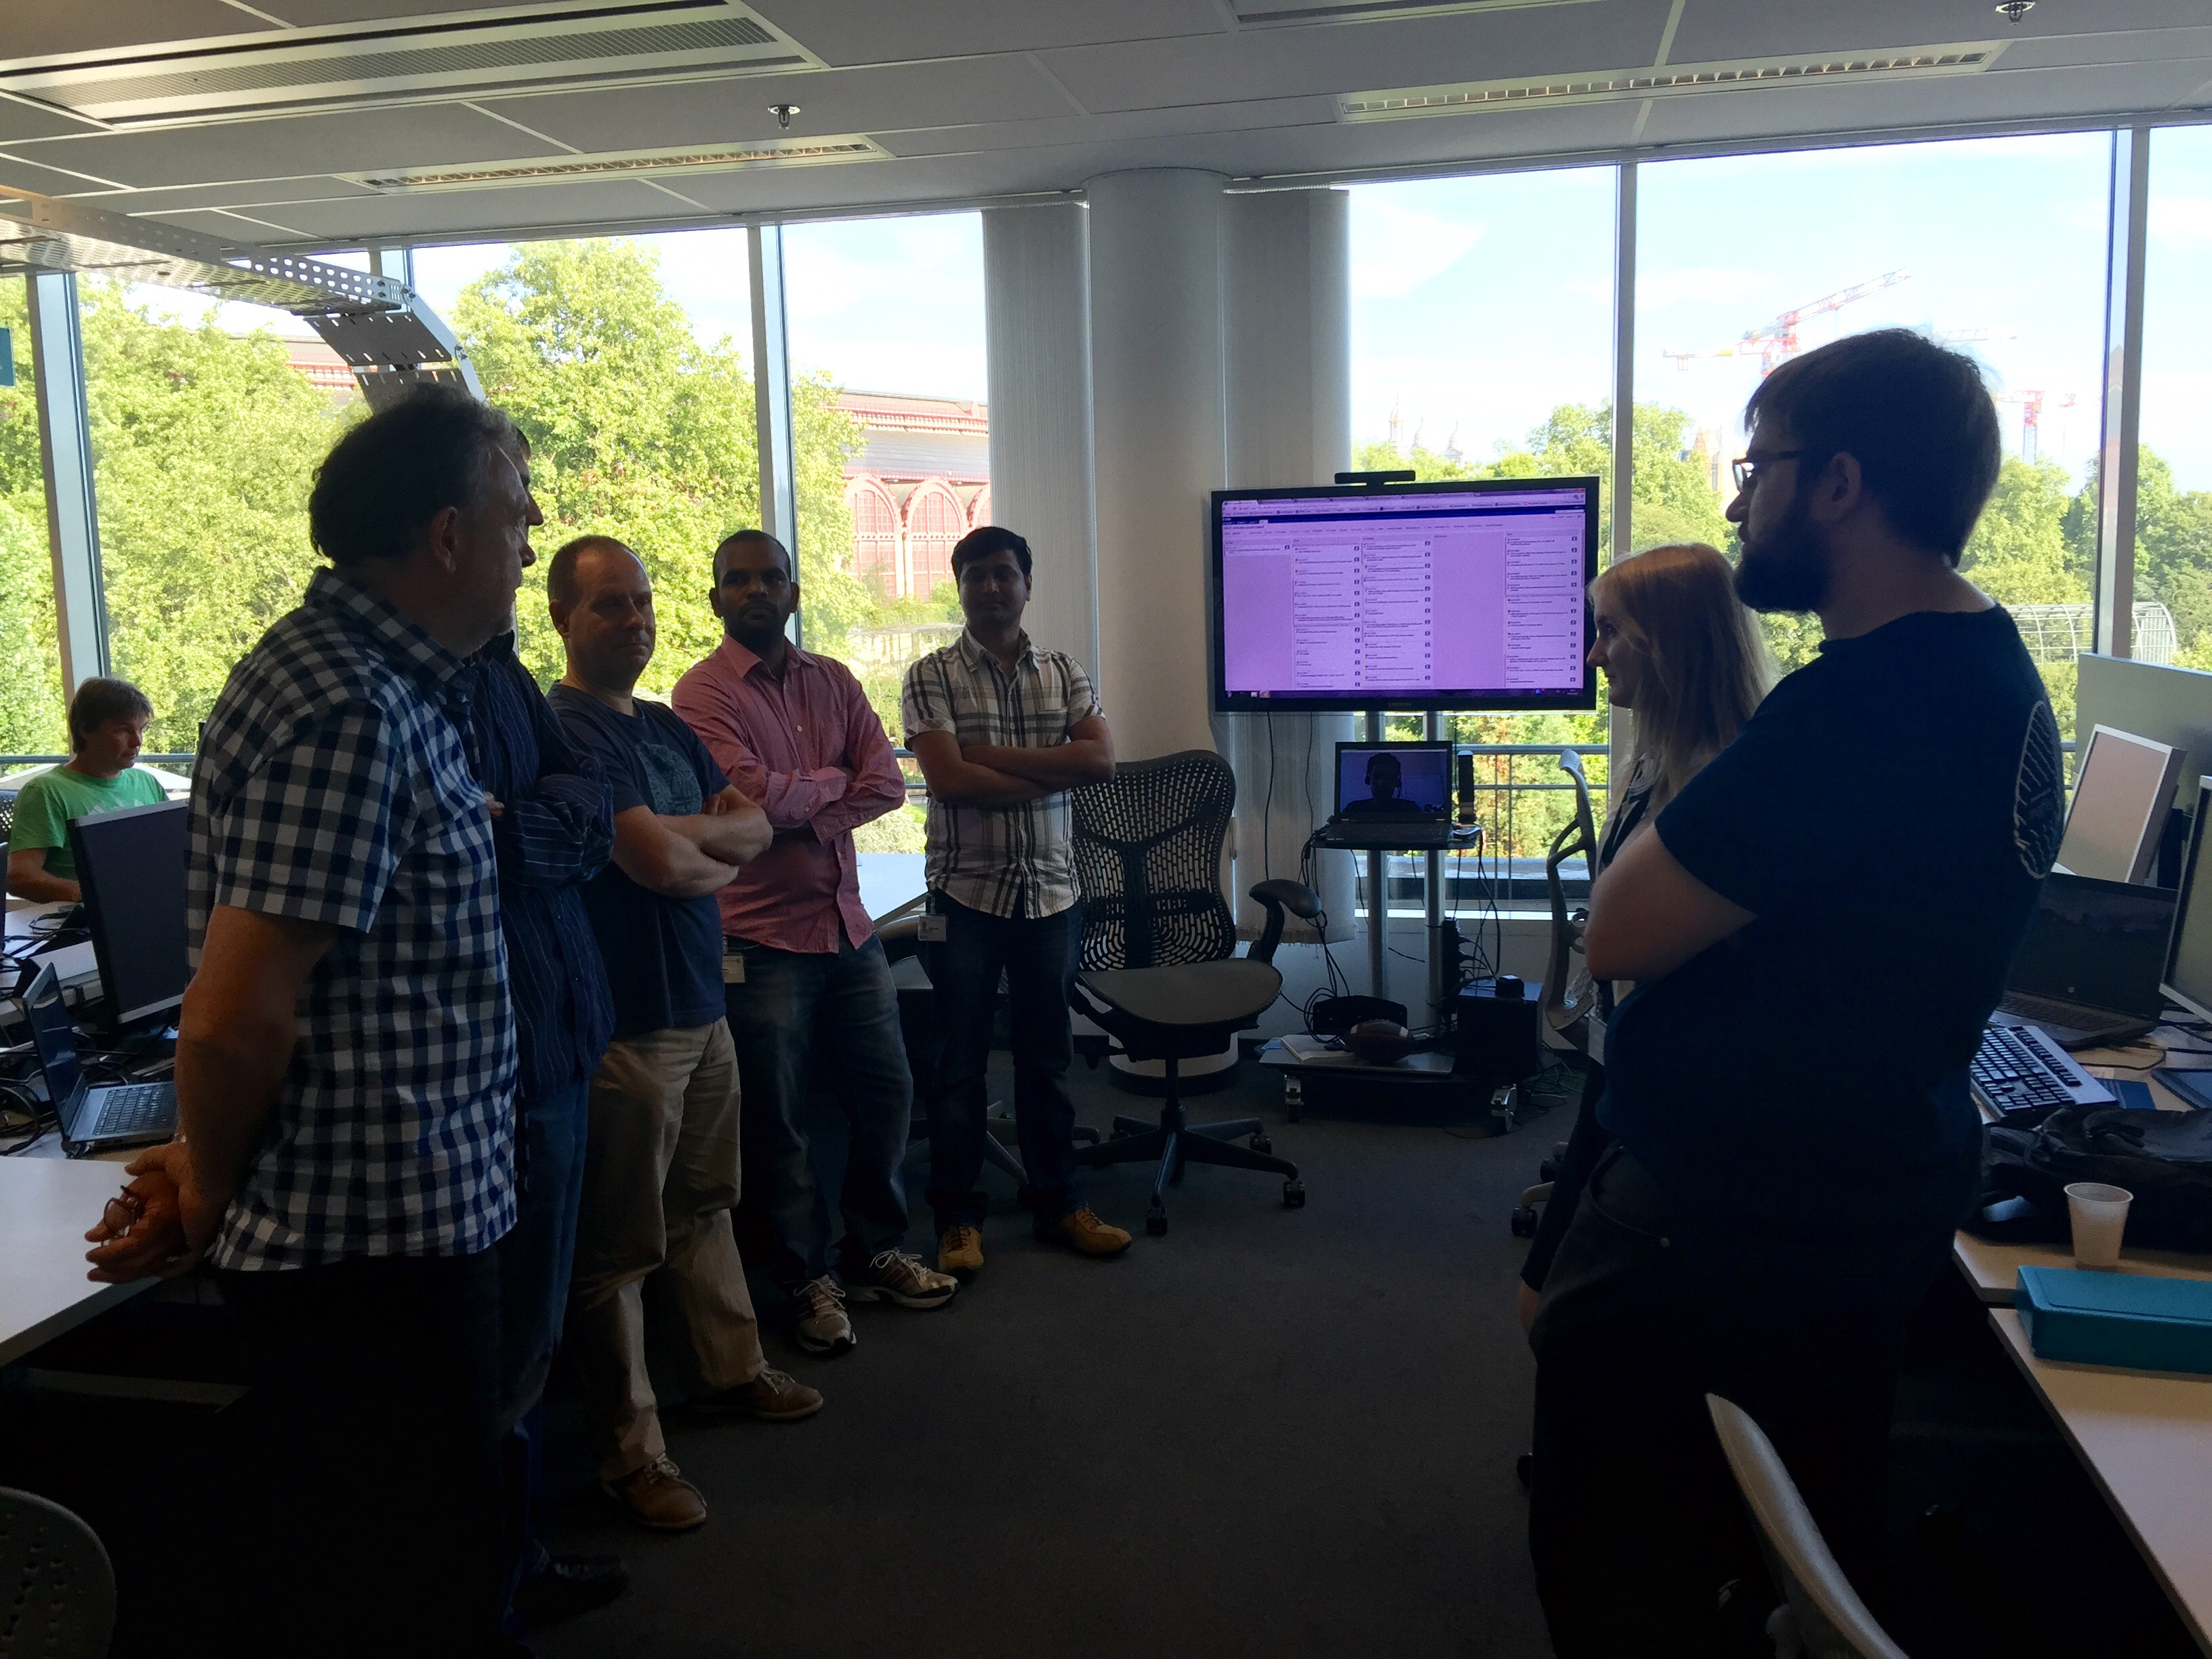
\includegraphics[width=60mm]{standupmeeting.jpg}
\caption{Een stand-up meeting van het NA-C team in Antwerpen.}
\label{standup}
\end{minipage}\hfill
\begin{minipage}{0.45\textwidth}
\centering
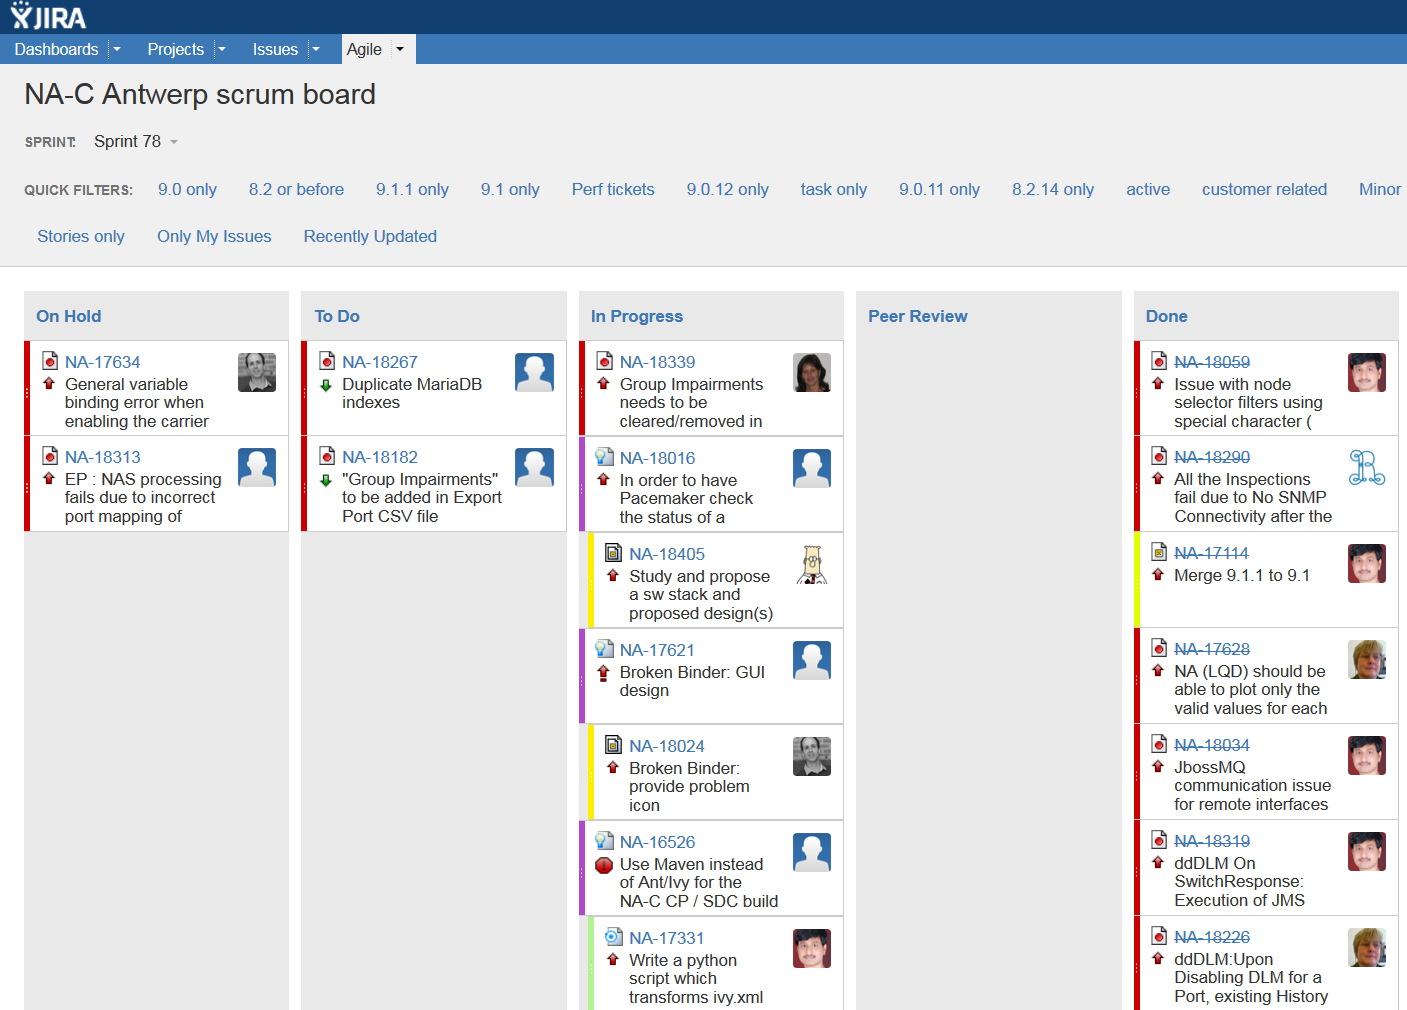
\includegraphics[width=60mm]{CaptureJira.png}
\caption{Het JIRA dashboard van het NA-C team in Antwerpen.}
\label{jira}
\end{minipage}
\end{figure}


In het NA-C team zijn er sprints van twee weken, wat wil zeggen dat er elke twee weken een evaluatie plaatsvindt van het werk dat in de afgelopen twee weken verzet is en waar besproken wordt welke veranderingen er naar de volgende sprint toe moeten doorgevoerd worden. Aan het begin van een sprint is er de sprint planning, waarin er bekeken wordt wat er moet gebeuren met welke prioriteit en wie wat gaat doen, op een heel algemeen niveau. Hierbij wordt gebruik gemaakt van \textit{user stories}, die een bepaalde taak omschrijven en de subtaken ervan. Het beschrijft wat de gebruiker nodig heeft bij het uitvoeren van zijn taak en bepaalt op deze manier wat er moet ontwikkeld worden om de gebruiker hierbij te helpen. Het omschrijft het ``wie", ``wat" en ``waarom" van deze vereisten op hoog niveau. Een voorbeeld van een \textit{user story} is te zien in Figuur \ref{user_story}. Aan het einde van de sprint is er de sprint \textit{review}, waarbij besproken wordt wat er bereikt is en waarbij eventueel demo's gegeven worden van wat er gerealiseerd is. Ook is er de sprint \textit{retrospective}, waarbij opgelijst wordt wat er goed en minder goed is gegaan, welke problemen er (binnen het team) waren en hoe die opgelost kunnen worden.

\begin{figure}[ht!]
\centering
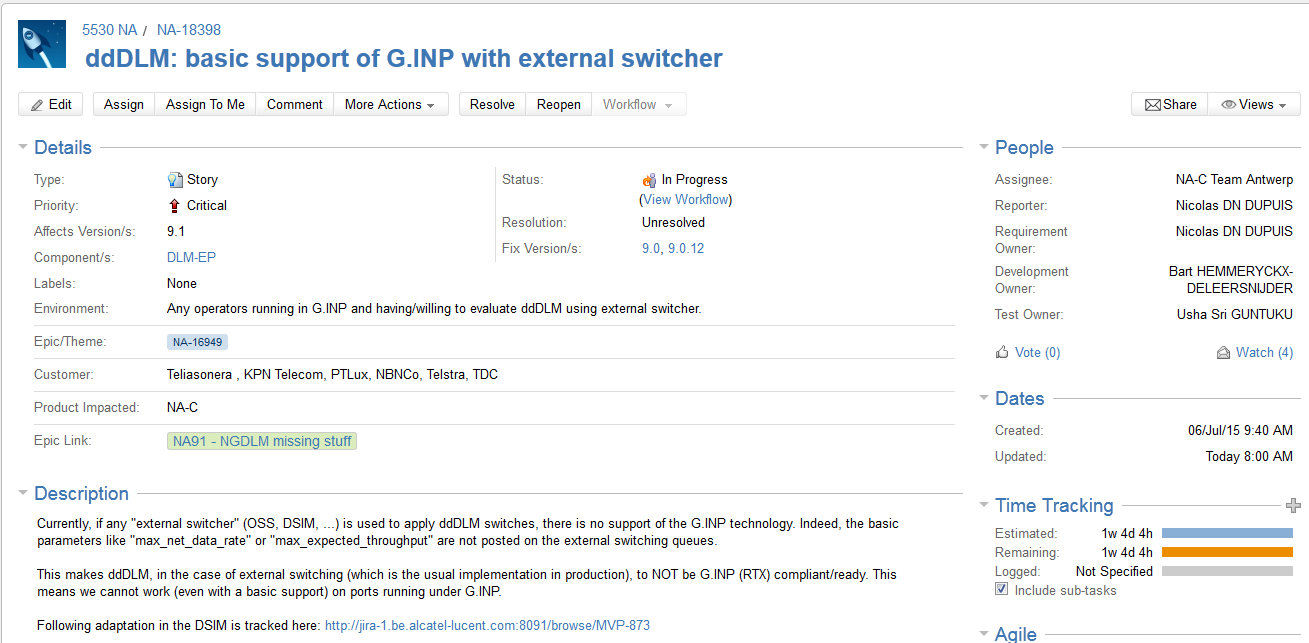
\includegraphics[width=90mm]{user_story.png}
\caption{Een van de \textit{user stories} van het team van NA-C in Antwerpen.} 
\label{user_story}
\end{figure}

\subsubsection{Continuous integration}
\label{ci}
Aangezien er regelmatig \textit{releases} van software zijn, wordt er gebruik gemaakt van \textit{continuous integration}, wat inhoudt dat wanneer iemand klaar is met het schrijven van een stuk code en deze \textit{commit}, alle \textit{builds} en testen hierrond automatisch zullen \textit{runnen} zodat fouten in een vroeg stadium kunnen gevonden en opgelost worden.\\
In Antwerpen wordt gebruik gemaakt van Jenkins\footnote{(2015, https://jenkins-ci.org/)}, een \textit{open-source continuous integration} systeem. Jenkins heeft een dashboard dat een overzicht toont van alle \textit{builds}, maar er kan ook gefilterd worden op zelfgemaakte criteria, zodat enkel de statussen van bepaalde \textit{builds} zichtbaar zijn. Een screenshot van dit dashboard is te zien in Figuur \ref{jenkins_orig}. Het overzicht van elke \textit{build} toont een gekleurde bol om aan te geven of de laatste \textit{build} geslaagd (groen of blauw) of gefaald (rood) is. Indien er testen gefaald zijn, dan zal de bol geel kleuren.
Er is ook een weerbericht dat toont hoe stabiel de \textit{build} is, waarbij slecht weer duidt op een instabiele \textit{build} en goed weer op een stabiele \textit{build}. 

\begin{figure}[ht!]
\centering
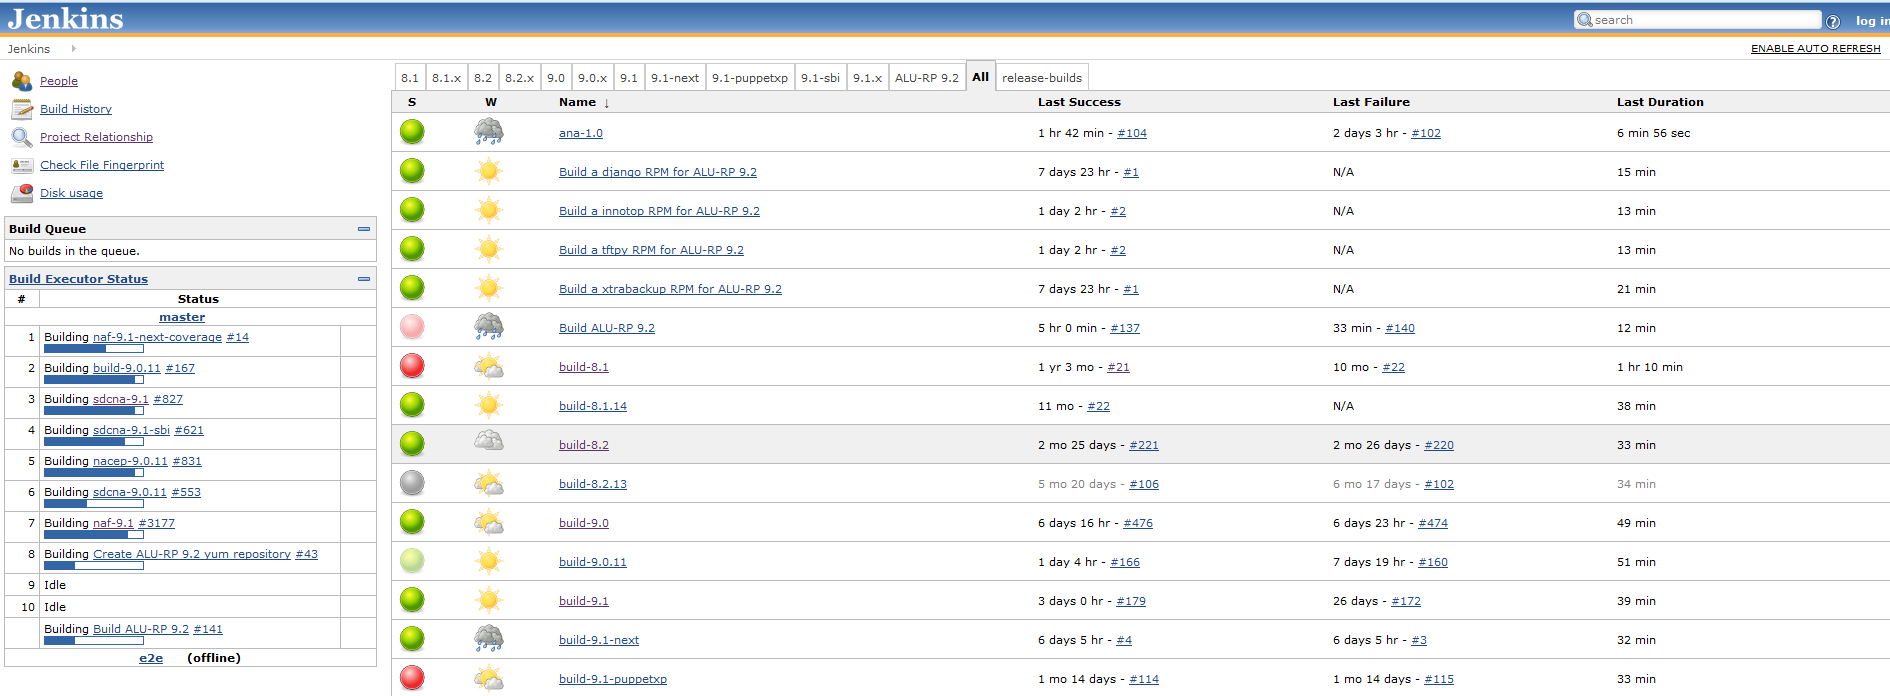
\includegraphics[width=90mm]{CaptureJenkins.png}
\caption{Het Jenkins dashboard, zoals oorspronkelijk gebruikt op de afdeling NA-C in Antwerpen.} 
\label{jenkins_orig}
\end{figure}

Het probleem met dit dashboard is dat het niet overzichtelijk is. De kleur van de bollen trekt wel de aandacht, maar het is vanop een afstand niet duidelijk welke \textit{builds} getoond worden. Het Jenkins dashboard wordt op de werkvloer weergegeven op een grote televisie, maar doordat het zo onoverzichtelijk is, wordt er niet naar gekeken. Zoals op Figuur \ref{tv_1} te zien is, is het zelfs op een groot scherm niet duidelijk welke \textit{builds} er getoond worden.

\begin{figure}[ht!]
\centering
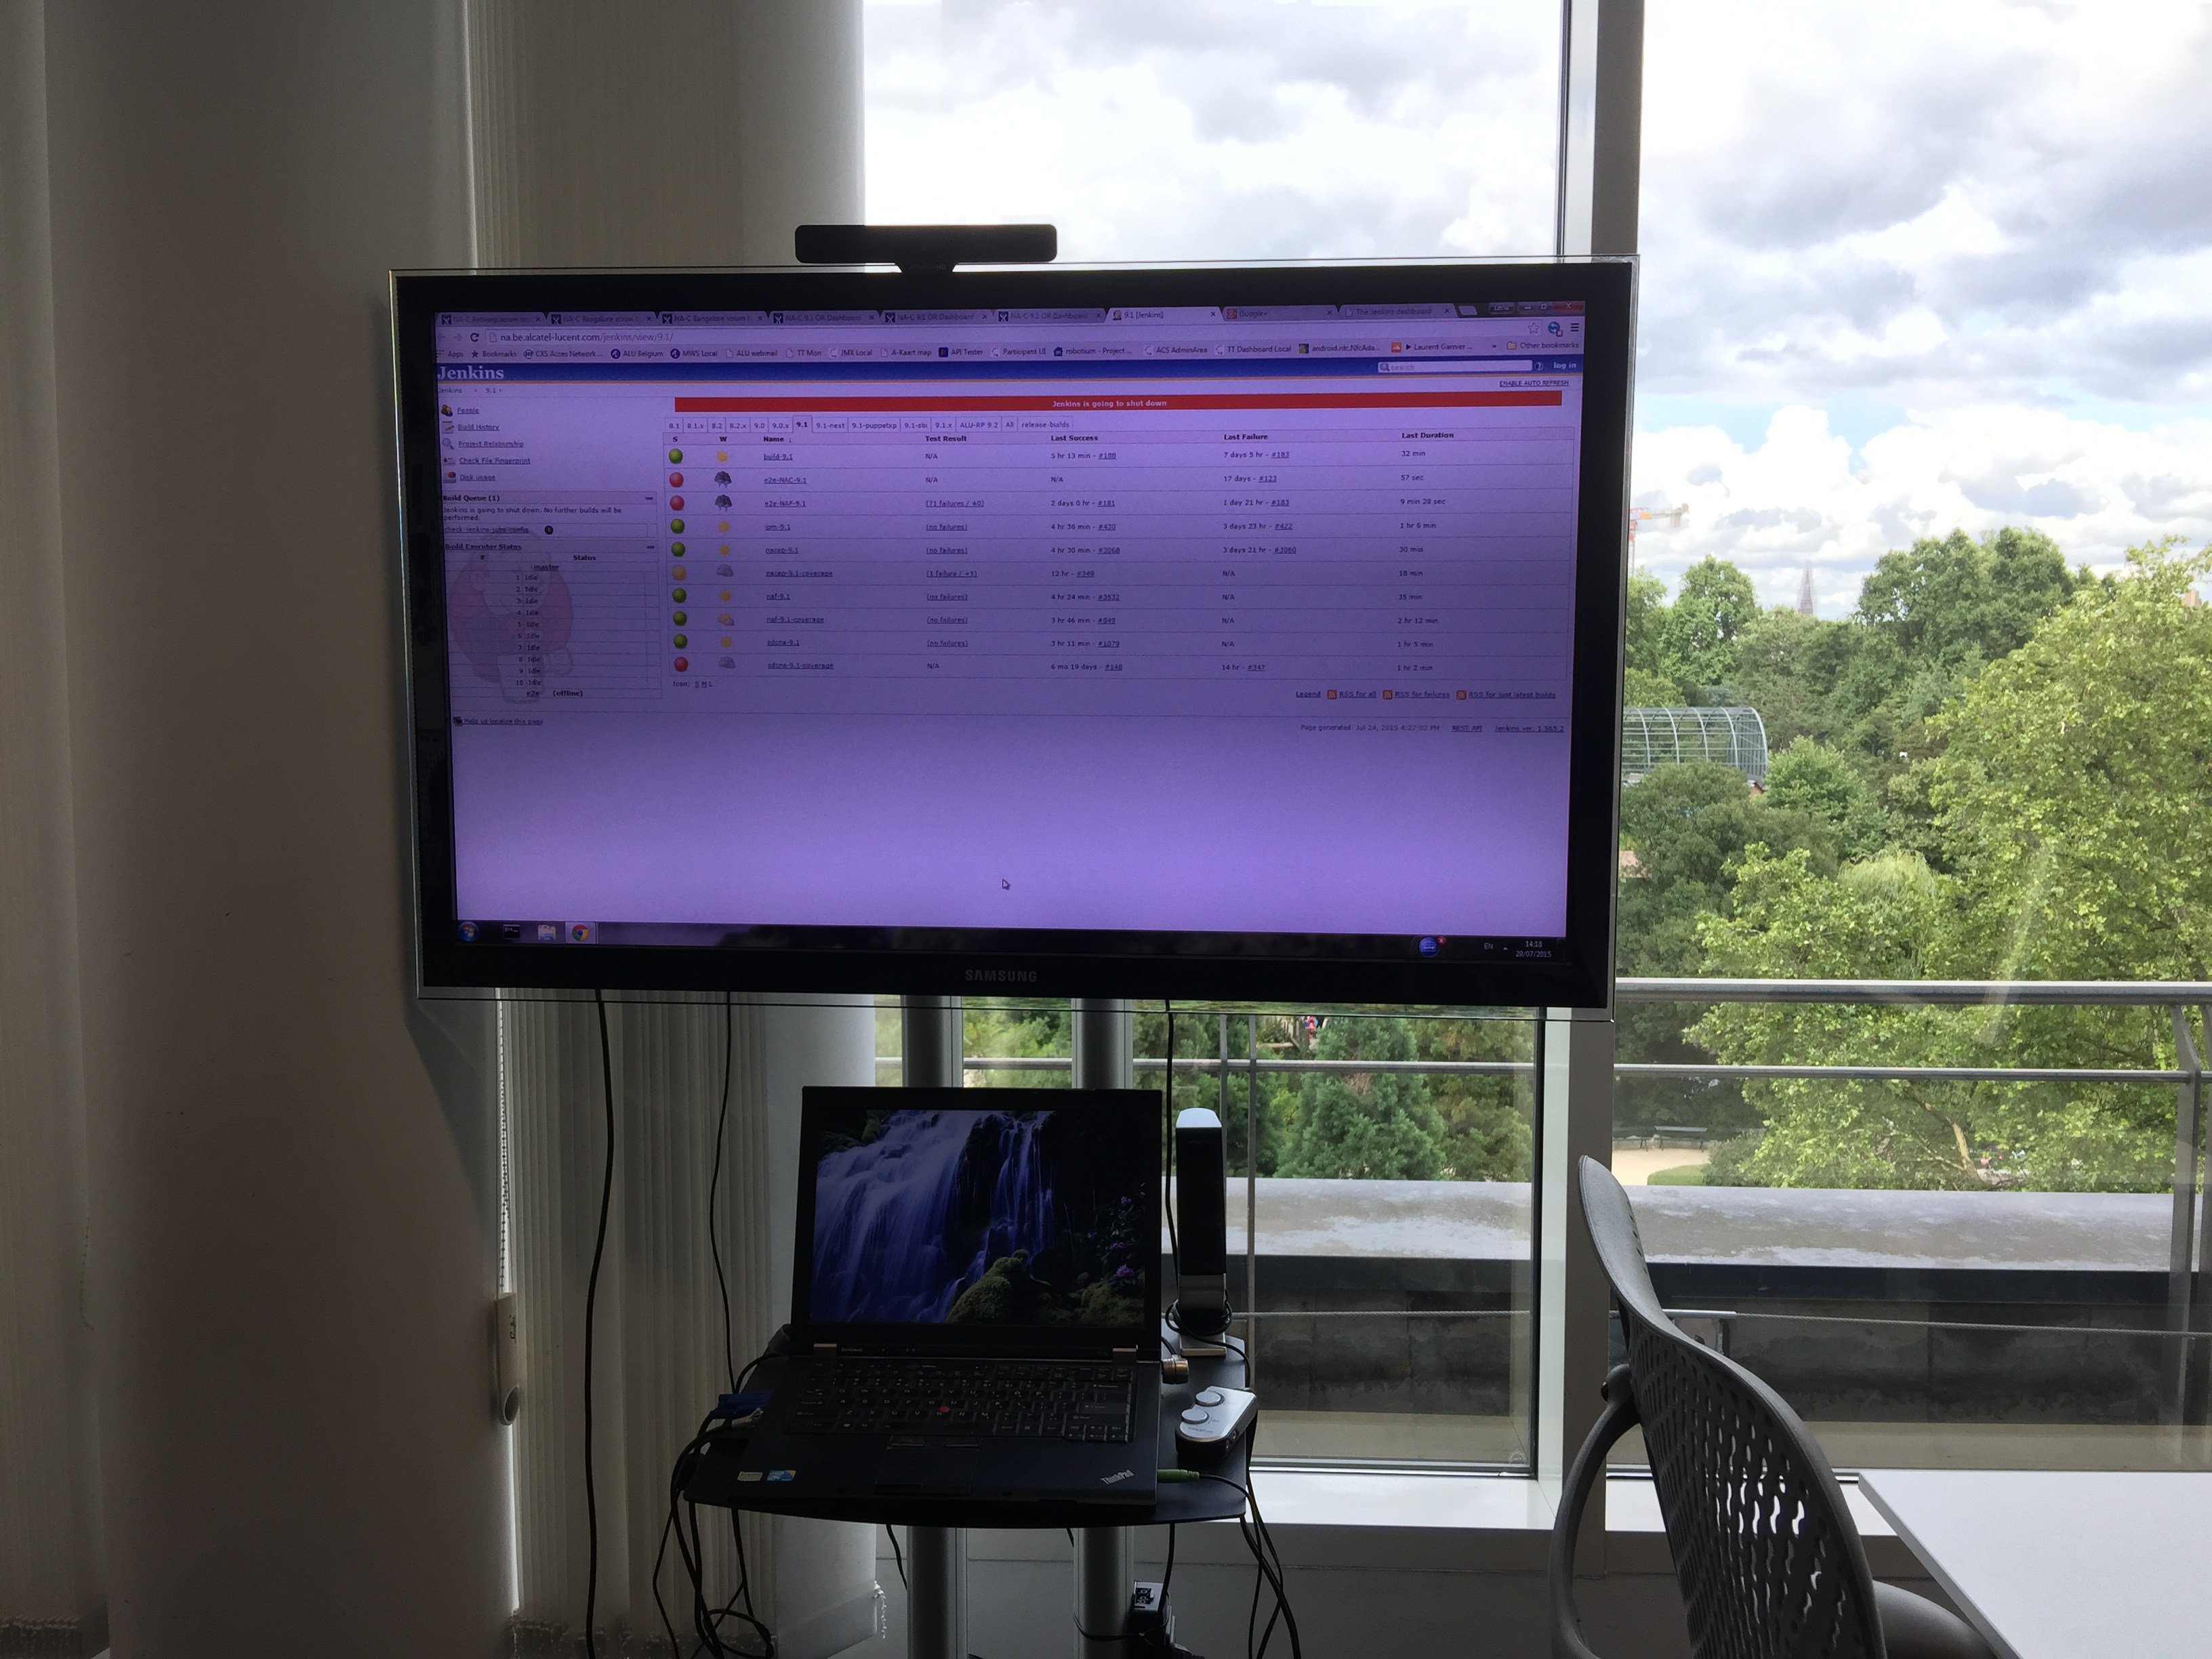
\includegraphics[width=90mm]{tvdashboardoriginal.jpg}
\caption{Het originele Jenkins dashboard weergegeven op de televisie op de afdeling van NA-C in Antwerpen.} 
\label{tv_1}
\end{figure}

\subsection{Stage-opdracht}
\label{opdracht}
De stage-opdracht bestond erin om ``Jenkins \textit{awareness}" te cre\"eren aan de hand van een dashboard dat een beter overzicht toont.
Wanneer gefaalde \textit{builds} meer in het oog springen, kan de code sneller herbekeken worden en is er echt sprake van \textit{continuous integration}. Gedurende heel de stage werd betrokkenheid gevraagd bij alles wat het team deed, zoals meedoen met de \textit{stand-up meetings} en het bijwonen van de sprint planning, de sprint \textit{review} en de sprint \textit{retrospective}, om zo een idee te vormen van hoe de \textit{agile} manier van werken toegepast wordt in een bedrijfsomgeving. Dat maakte duidelijk hoe deze manier van werken een team sterker kan maken, gezien iedereen weet wie waarmee bezig is en hoe de korte evaluatieperiodes ervoor zorgen dat er kort op de bal gespeeld kan worden.\\
Voor de stage-opdracht werd een apart project gemaakt, waarbij er ook gewerkt werd volgens de \textit{agile}-methode met tweewekelijkse sprints. Er werd voor het project een JIRA-pagina aangemaakt, waarop de vooruitgang werd bijhouden door taken aan te maken die  moesten uitgevoerd worden en waar problemen gerapporteerd werden. Een screenshot van dit JIRA-dashboard is te zien in Figuur \ref{my_jira}.
De eerste sprint bestond uit het maken van een literatuurstudie, te vinden in Appendix \ref{lit_study}. Hierin wordt onderzocht waarop gelet moet worden bij het maken van een (goed) dashboard en wat er verbeterd kan worden aan het originele Jenkins dashboard. Vervolgens zijn enkele voorstellen voor dashboard-layouts opgemaakt en is er een kleine enqu\^ete uitgevoerd binnen het team, om te kijken welke voorkeuren zij hadden. Hierop wordt dieper ingegaan in sectie \ref{sprint1}.\\
Tijdens de tweede sprint is het dashboard ontwikkeld en voorgesteld aan de NA-C teams in Antwerpen, Chennai en Bangalor. Dit proces is te vinden in sectie \ref{sprint2}.\\
De derde en laatste sprint bestond uit het voeren van een enqu\^ete over de huidige versie van het dashboard, om het vervolgens te verbeteren. In de tweede helft van deze sprint is het dashboard in gebruik genomen op de Jenkins \textit{server} van Alcatel-Lucent. Dit wordt besproken in sectie \ref{sprint3}.

\begin{figure}[ht!]
\centering
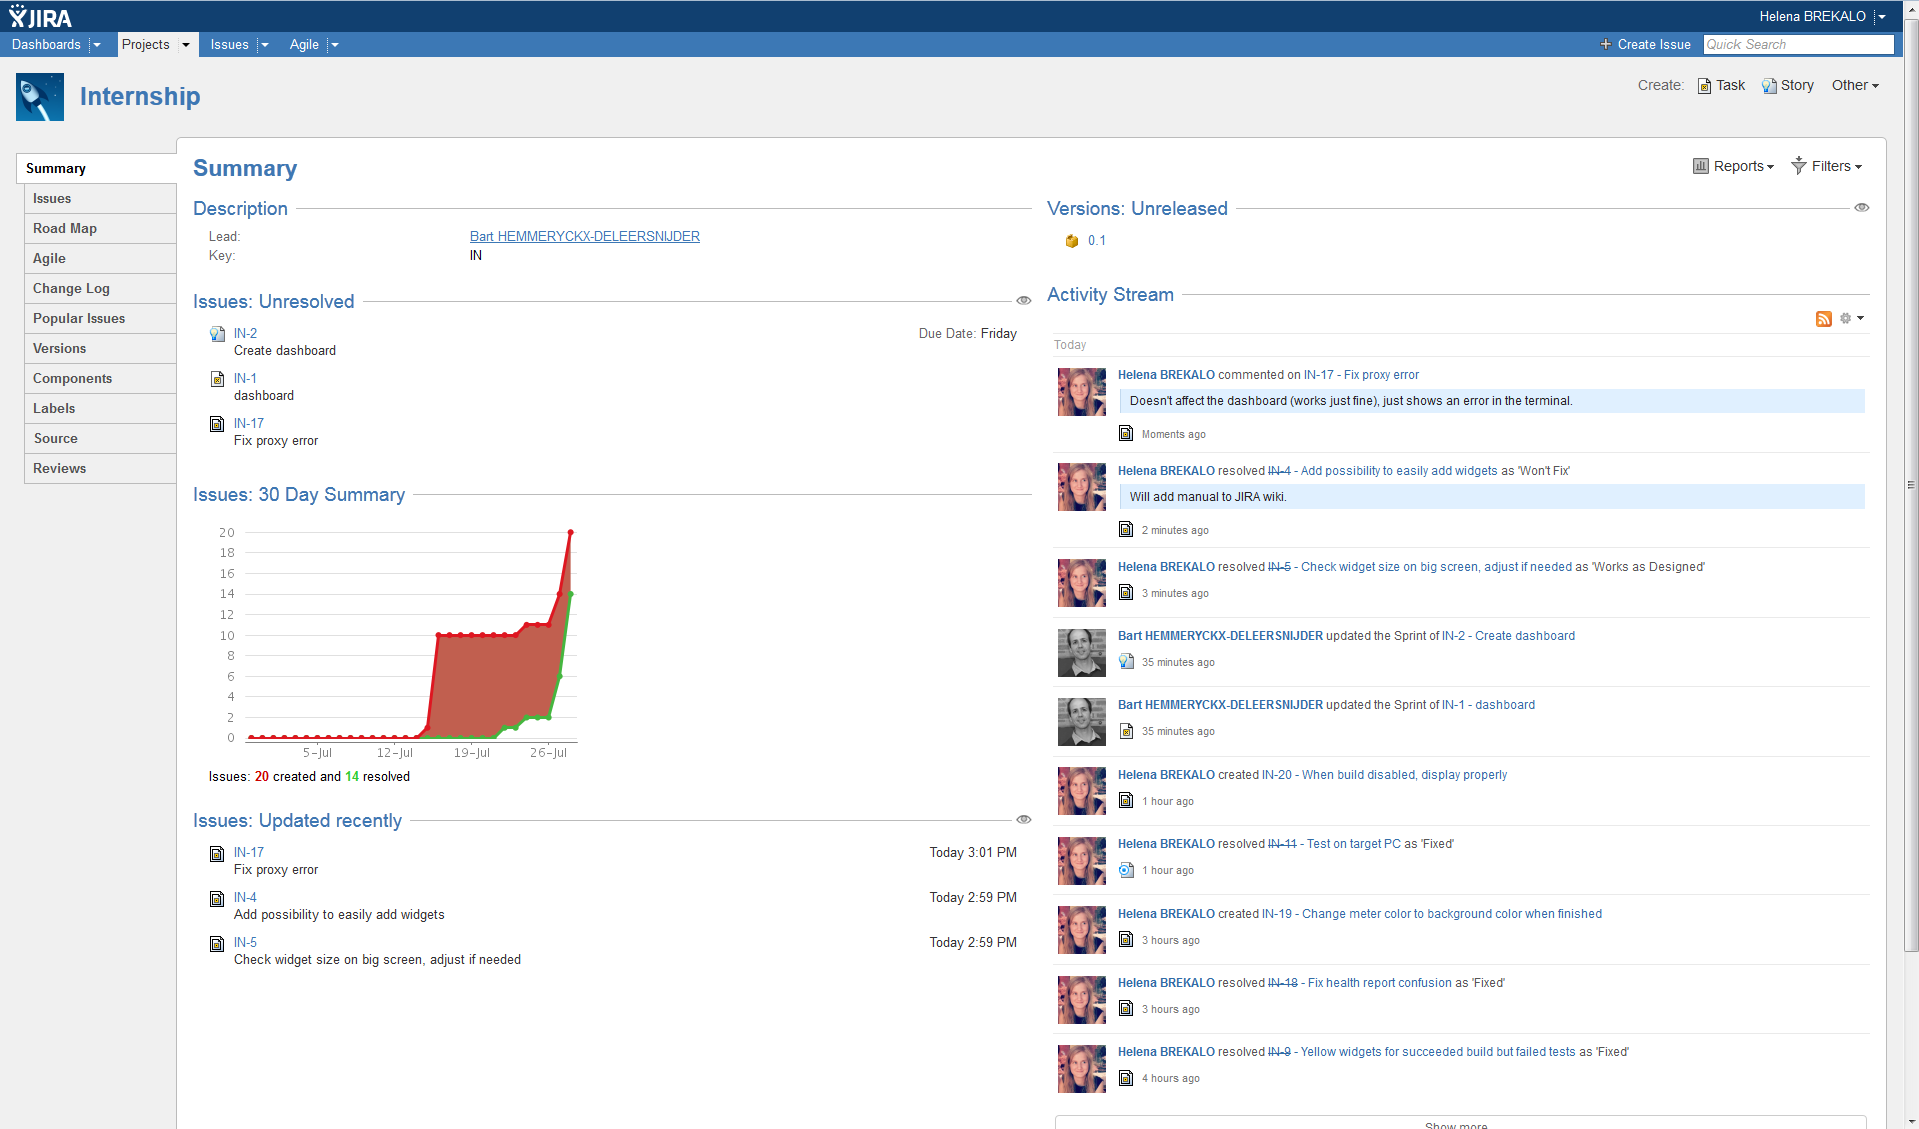
\includegraphics[width=90mm]{myJIRAscreenshot.png}
\caption{Het JIRA-dashboard voor mijn stage.} 
\label{my_jira}
\end{figure}

\subsubsection{Sprint 1: Onderzoek en literatuurstudie} 
\label{sprint1}
\paragraph{Literatuurstudie} Tijdens de eerste sprint is er onderzoek gevoerd naar hoe goede dashboards eruit zien en hoe ze overzichtelijk gehouden kunnen worden. Hierrond is een literatuurstudie gemaakt, die gevonden kan worden in Appendix \ref{lit_study}. Uit deze literatuurstudie bleek dat het voorziene Jenkins dashboard niet voldeed aan veel van de vereisten, aangezien de belangrijkste informatie niet \'e\'en oogopslag zichtbaar is.\\
Naast het maken van de literatuurstudie is er ook bekeken welke \textit{tools} er zijn om dashboards te maken, waarbij Dashing\footnote{(2015, http://dashing.io/)} aangeraden werd door een collega. Na het bekijken van enkele andere \textit{tools} om dashboards te ontwikkelen, is er uiteindelijk voor Dashing gekozen, aangezien het enorm veel flexibiliteit biedt.
\paragraph{Enqu\^ete}
Na het onderzoek en de literatuurstudie is er een voorstel voor dashboardontwerpen opgemaakt die werd voorgelegd aan het team bij NA-C in Antwerpen. Hierbij hoorde een enqu\^ete waarbij gekozen kon worden voor verschillende ontwerpen en waarbij opmerkingen gegeven konden worden. Uit die opmerkingen zijn nog nuttige commentaren gekomen, waarbij enkele van die idee\"en ook in het dashboard verwerkt zijn. De enqu\^ete en de resultaten zijn te vinden in Appendix \ref{enquete1}. 
\subsubsection{Sprint 2: Ontwikkeling dashboard} 
\label{sprint2}
Op het einde van de eerste sprint vond een \textit{sprint review} en \textit{sprint retrospective} plaats, om de gemaakte vooruitgang te evalueren. Deze meeting werd gecombineerd met de sprint planning, waar een eerste versie van het ontwerp en de \textit{tools} voor het dashboard werden voorgesteld.
\paragraph{Gebruikte \textit{tools}}
Dashing is een dashboard \textit{framework} dat geschreven is in Sinatra, een \textit{open source} software web applicatie geschreven in Ruby. De ontwikkeling gebeurde in Linux, waarbij gebruik gemaakt werd van Ubuntu 14.04. Op deze PC is een lokale Jenkins-omgeving opgezet, zodat het dashboard tijdens de ontwikkeling hiermee getest kon worden. Het schrijven van de code gebeurde in gedit en debuggen gebeurde via de \textit{terminal}.\\
De ``tegels" op het dashboard worden omschreven als \textit{widgets} waarbij je verschillende soorten \textit{widgets} kan hebben, met elk een bepaalde functionaliteit. Tijdens deze fase van het project werd er gefocust op een \textit{widget} om informatie over Jenkins te tonen. Deze \textit{widget} kan gebruikt worden voor verschillende \textit{builds}, het is niet de bedoeling om voor elke \textit{build} een nieuw \textit{widget} te ontwikkelen, tenzij je andere informatie wilt tonen op de verschillende Jenkins-\textit{widgets}. Tijdens de derde sprint is hier nog een \textit{widget} voor \textit{RSS-feeds} aan toegevoegd, zodat ook het meest recente nieuws gevolgd kan worden.
\paragraph{Gebruikte talen}
Het schrijven van het dashboard is gebeurd in verschillende talen, hieronder een opsomming welke taal gebruikt werden.
\begin{description}
\item[HTML] HTML wordt gebruikt om te bepalen hoe de inhoud getoond wordt op de \textit{widget}, dus bijvoorbeeld welk deel als titel zal getoond worden en welke onderdelen als paragrafen weergegeven worden. HTML bepaalt ook de locatie van de elementen op de \textit{widget}. De informatie die getoond wordt, wordt via Batman Bindings\footnote{(Small, 2013, http://batmanjs.org/)} uit de JSON data van de Jenkins server \textit{geparset}.
\item[(S)CSS] CSS wordt gebruikt om de tekst uit het HTML-bestand op te maken (grootte van de tekst, stijl, kleur,...), waarbij SCCS (Sassy CSS) ervoor zorgt dat je ook variabelen kan gebruiken, wat niet mogelijk is in standaard CSS. Op deze manier kan code van een bepaalde opmaak hergebruikt worden via variabelen. 
\item[Javascript] Javascript werd gebruikt in de Batman Bindings, die ervoor zorgen dat de data die van de website \textit{geparset} wordt, dynamisch gebruikt kan worden in de HTML-bestanden. Op zich is de Batman Bindings-\textit{library} klaar om te gebruiken, maar om een tijdstip te \textit{parsen} (dat werd weergegeven als Unix \textit{timestamp}), is gebruik gemaakt van de moment.js-\textit{library}.
\item[Coffeescript] Coffeescript is een taal die transcompileert naar Javascript. Het .coffee-bestand voor een \textit{widget} specifi\"eert hoe de data, die via het HTML-bestand opgevraagd wordt, weergegeven wordt. Dit bestand was van belang om onder andere het juiste weerbericht te tonen. Het coffeescript parset de data die via de Batman Bindings werd opgehaald en geeft aan hoe die doorgegeven wordt aan het HTML-bestand. Zonder het .coffee-bestand zou er enkel \textit{plain text} (mits wat opmaak door CSS) te zien zijn op de \textit{widget}.
\item[Ruby] Dashing maakt gebruik van Embedded Ruby om te bepalen welke tegels getoond worden op het dashboard en van \textit{plain} Ruby om de data op te halen en te \textit{parsen} vanuit de juiste plaats (nl. de Jenkins server) via de JSON-data die werd voortgebracht hierdoor. Ook wordt hier de link gelegd tussen de \textit{build jobs} die getoond \emph{kunnen} (niet per s\'e zullen\footnote{Welke build jobs getoond worden, wordt bepaald door de Embedded Ruby file.}) worden op het dashboard.
\item[JQuery] JQuery wordt gebruikt in het coffeescript bestand om CSS-gewijs klassen of ID's te gebruiken van elementen waarop een bepaalde actie moet uitgevoerd worden. Er is van JQuery gebruik gemaakt om de \textit{build} meter te doen verschijnen en verdwijnen bij het starten of aflopen van een \textit{build} en om het weerbericht en de status vand e \textit{build} te tonen.
\item[JSON] JSON wordt gebruikt om de data uit van de Jenkins server te \textit{parsen}, zodat die opgevraagd kan worden in het Ruby bestand.
\end{description}
Er is gebruik gemaakt van Codecademy\footnote{(2015, https://www.codecademy.com/)} en online \textit{tutorials} om basiskennis te verwerven van de gebruikte talen.\\

De verschillende bestanden worden als volgt gebruikt:
\begin{itemize}
\item Een \textit{widget} wordt opgesteld door middel van een .HTML-bestand, een .scss-bestand en een .coffee-bestand.
\item Een Embedded Ruby bestand geeft via HTML-\textit{blocks} aan welke \textit{build} jobs getoond worden op het dashboard.
\item Een \textit{plain} Ruby bestand doet de \textit{mapping} van de JSON-data op de variabelen in het dashboard en defini\"eert de namen van de \textit{build} jobs die getoond kunnen worden.
\end{itemize}
\paragraph{Sprint Review} Op het einde van de tweede sprint is de eerste versie van het dashboard gedemonstreerd voor het team in Antwerpen, Bangalor en Chennai\footnote{De presentatie is te vinden in Appendix \ref{ppt}}. Er kon een werkend dashboard getoond worden dat informatie weergeeft over de Jenkins \textit{build} jobs die op een lokale \textit{server} draaiden. De feedback hierop was positief en enkele vragen van mensen in de verschillende teams konden beantwoord worden.
\subsubsection{Sprint 3: Feedback en verbetering}
\label{sprint3}
Na de sprint review is de Alcatel-Lucent Jenkins-server ge\"integreerd in het dashboard, wat nog anderhalve dag van \textit{debugging} vroeg, gezien de Jenkins-server nu niet lokaal draaide, maar op een andere server (nl. de Jenkins-server van het NA-C team in Antwerpen). Ook gebruikt men bij Alcatel-Lucent een andere versie van Jenkins, waardoor bepaalde sleutelwoorden waarop \textit{geparset} wordt anders heten.\\
Na de sprint \textit{retrospective} van sprint 2 en de sprint planning van sprint 3 is er nog een enqu\^ete uitgevoerd om positieve en negatieve commentaren te verzamelen. De resultaten van deze enq\^ete zijn te vinden in Appendix \ref{enquete2}.
Een van de uitbreidingen die zijn gemaakt is het tonen van een \textit{RSS-feed} dat nieuws weergeeft. Ook is het dashboard aangepast zodat de meter van de \textit{build} status verdwijnt wanneer de \textit{build} compleet is. Enkele screenshots van het dashboard uit de derde sprint zijn te zien in Sectie \ref{resultaat}.
\paragraph{Ingebruikname} \todo{over vertellen}
\subsection{Resultaat}
\label{resultaat}
\paragraph{Resultaat na sprint 2}
De eerste versie van het dashboard is te zien in Figuur \ref{dash_1}. Het dashboard in zijn huidige vorm is gemaakt om getoond te worden op een HD-scherm met 16:9-ratio. Het is de bedoeling dat er zes tegels naast elkaar kunnen staan en dat er drie rijen zijn, wat maakt dat de status van 18 \textit{build} jobs gelijktijdig getoond kunnen worden. Dit bleek ruim voldoende voor het NA-C team, aangezien er altijd maar op enkele \textit{builds} tegelijkertijd gefocust wordt.

\begin{figure}[ht!]
\centering
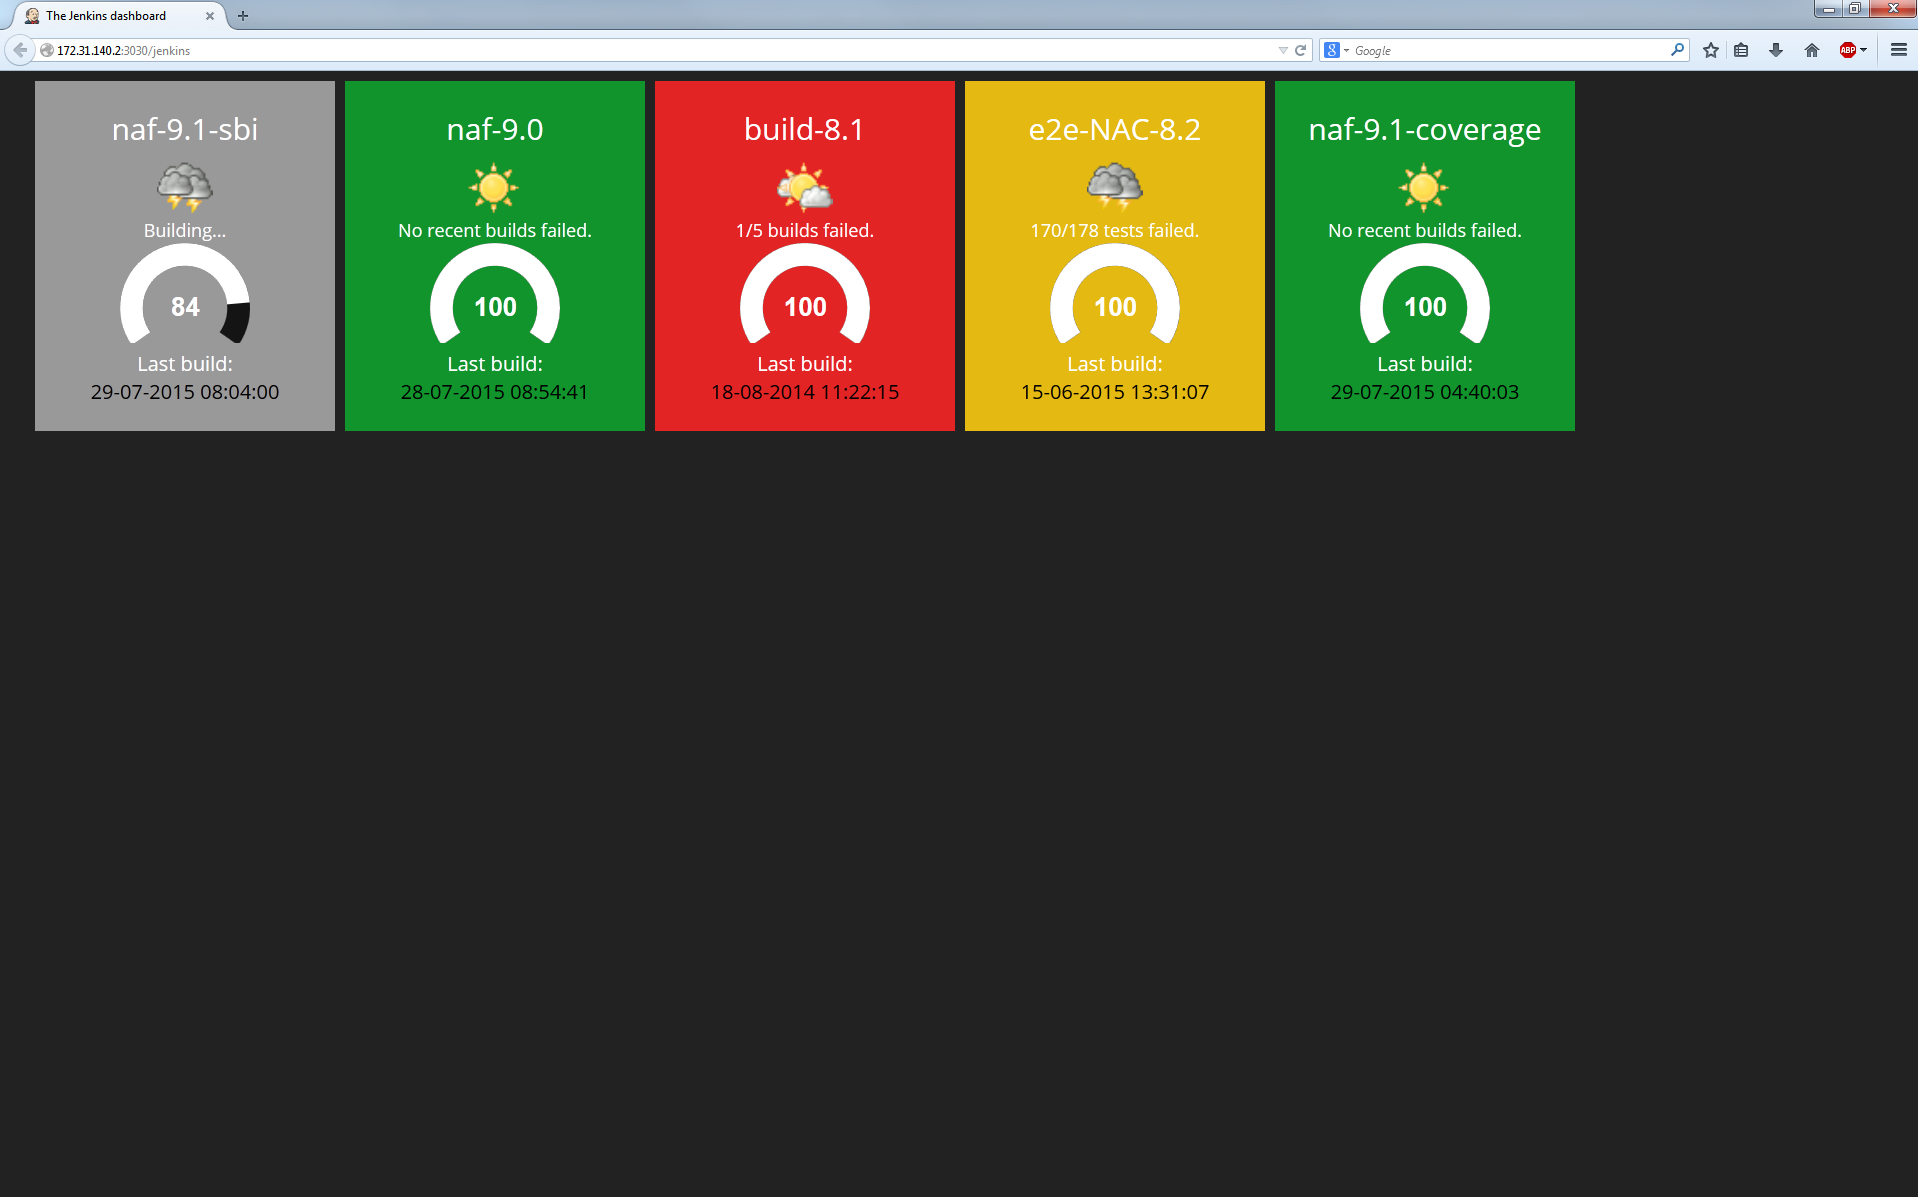
\includegraphics[width=90mm]{dashboard_screenshot1.png}
\caption{Eerste versie van het dashboard.} 
\label{dash_1}
\end{figure}

Figuur \ref{dash_2} toont de tegels in meer detail. De titel is de naam van de \textit{build} waarover de tegel informatie verschaft. Het weerbericht toont de stabiliteit van de \textit{build}, of, indien er testen gefaald zijn, de stabiliteit van de testen. De tekst eronder geeft aan hoe stabiel de \textit{builds} of de testen zijn, de meter geeft aan hoe ver de \textit{build} gevorderd is het tijdstip daaronder toont wanneer de laatste \textit{build} uitgevoerd is.\\
Er zijn verschillende achtergrondkleuren gebruikt die de status van de laatste \textit{build} weergeven:
\begin{itemize}
\item Grijs: de \textit{build} is nog bezig, het weerbericht toont de stabiliteit van de \textit{builds} van voor degene die nu bezig is.
\item Rood: de laatste \textit{build} is gefaald.
\item Geel: \'e\'en of meerdere testen zijn gefaald.
\item Groen: de laatste \textit{build} is geslaagd en alle testen zijn geslaagd. 
\end{itemize}
Als er gekeken wordt naar het voorstel opgemaakt in de literatuurstudie is de achtergrondkleur daar niet aanwezig (de \textit{\textit{build} status} wordt er weergegeven met een gekleurde bol), maar de enqu\^ete bij NA-C in Antwerpen toonde dat iedereen te vinden was voor de gekleurde achtergrond.

\begin{figure}[ht!]
\centering
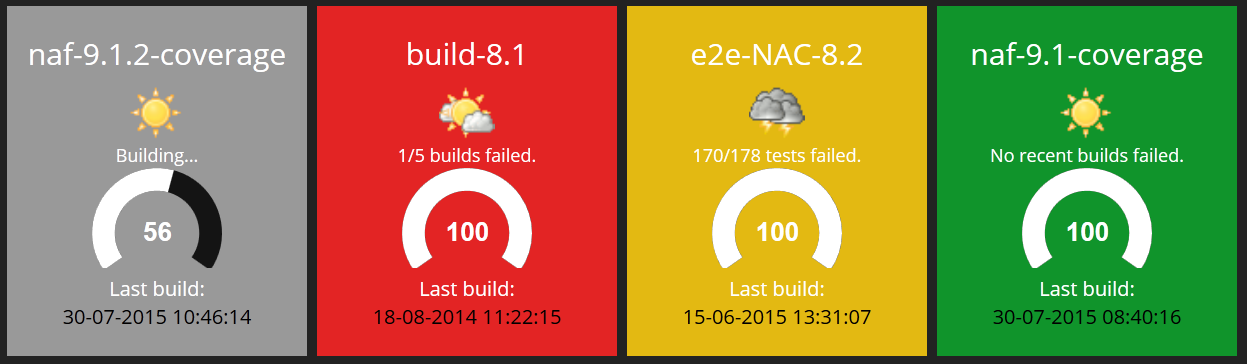
\includegraphics[width=90mm]{screenshot2.png}
\caption{Gedetailleerd overzicht dashboard.} 
\label{dash_2}
\end{figure}

\paragraph{Resultaat na sprint 3}
Na de tweede enqu\^ete (te vinden in Appendix \ref{enquete2}) zijn nog enkele veranderingen doorgevoerd. De belangrijkste zijn:
\begin{itemize}
\item De meter verdwijnt wanneer de \textit{build} niet bezig is, zo leidt deze de aandacht niet onnodig af.
\item Er is een \textit{RSS-feed} toegevoegd voor nieuwsitems.
\item Er kunnen zones van \textit{widgets} gecre\"eerd worden, om te tonen welke samen horen. In Figuur \ref{dash_3} is dit gedaan met de nieuwsitems, maar het kan dus ook perfect met de \textit{build widgets}.
\end{itemize}

Er zijn ook twee nieuwe kleuren van \textit{widgets} toegevoegd:
\begin{itemize}
\item Zwart: de desbetreffende \textit{build} is uitgeschakeld (\textit{disabled}). Er wordt op deze \textit{widget} geen weerbericht getoond, wel het tijdstip waarop de laatste \textit{build} is uitgevoerd.
\item Lichtblauw: deze kleur is bedoeld voor de nieuws\textit{widget}, om deze duidelijk te kunnen onderscheiden van de Jenkins \textit{widgets}.
\end{itemize}

Het finale resultaat is te zien in Figuur \ref{dash_3}. Op Figuur \ref{dash_4} is het dashboard te zien op de televisie van de afdeling NA-C. Figuur \ref{dash_5} toont de finale versie van het dashboard in meer detail.

\begin{figure}
\centering
\begin{minipage}{0.45\textwidth}
\centering
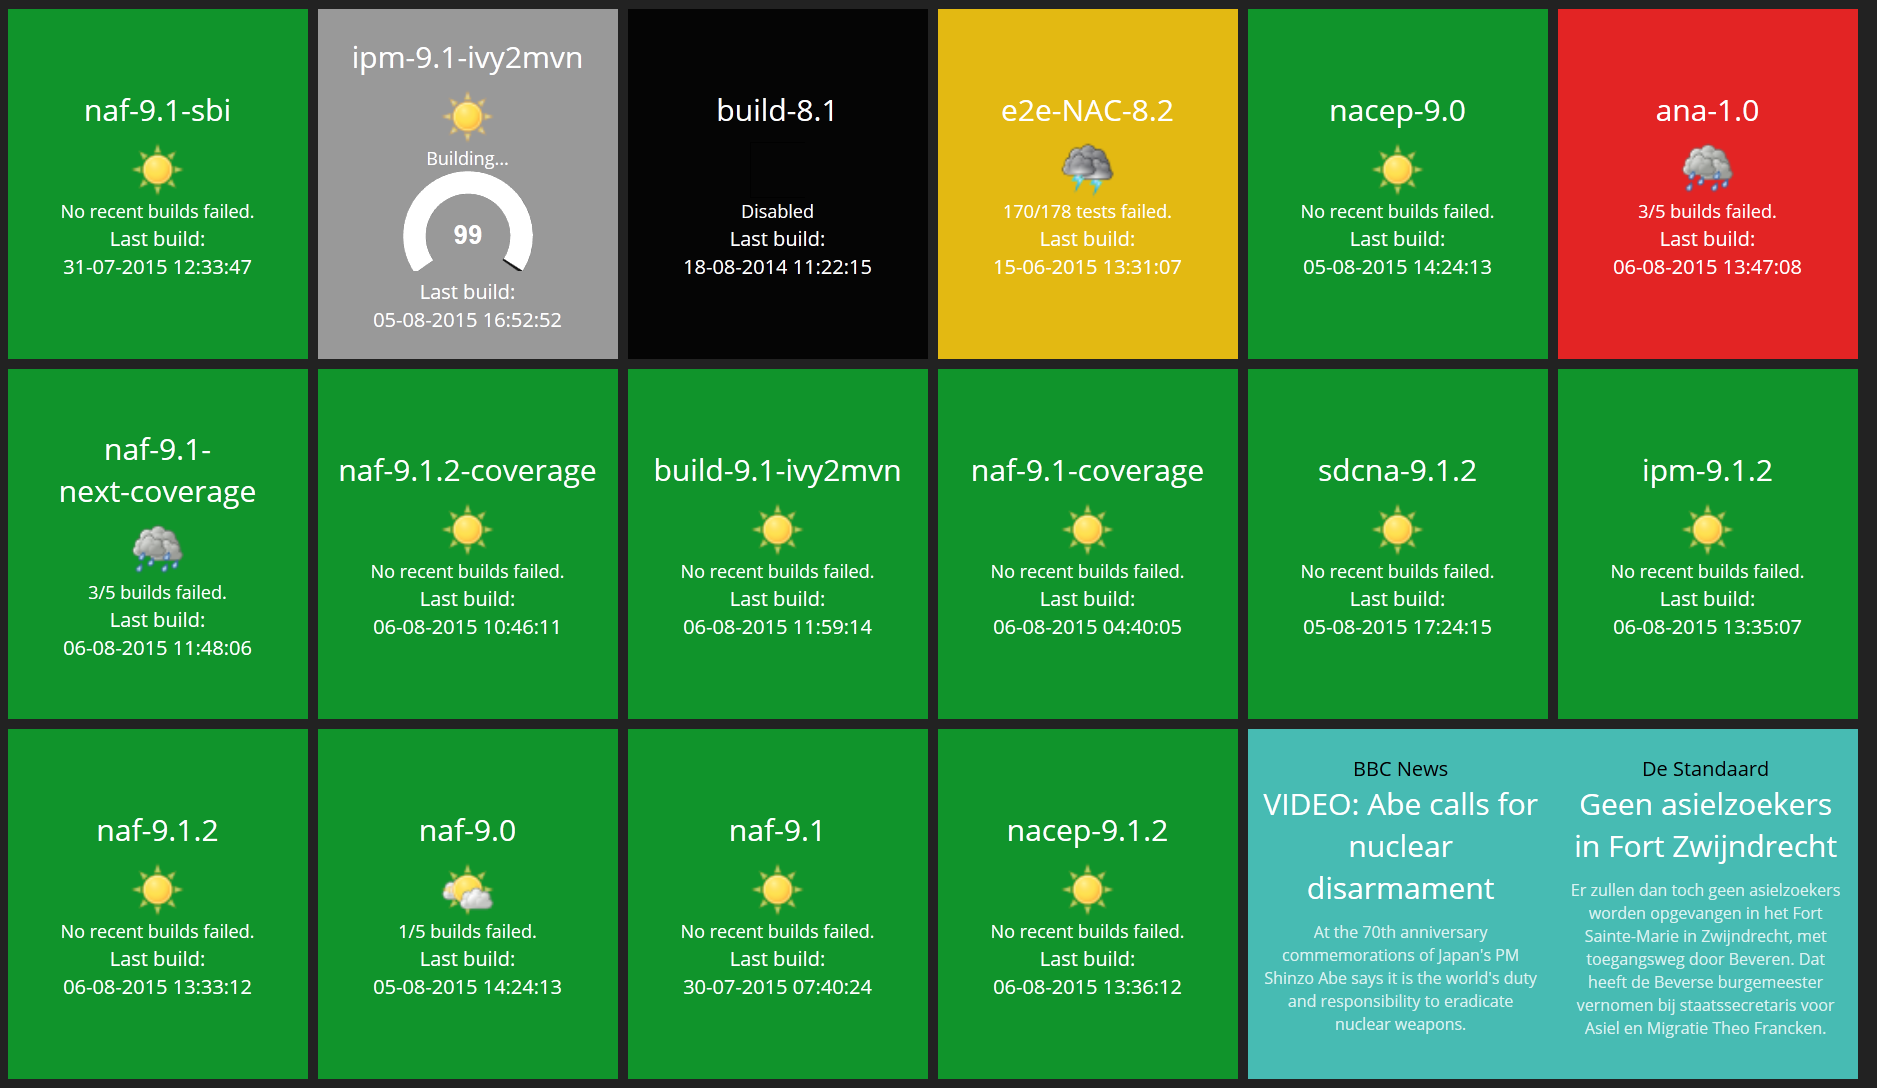
\includegraphics[width=60mm]{dashboard_screenshot4.png}
\caption{Finale versie dashboard.}
\label{dash_3}
\end{minipage}\hfill
\begin{minipage}{0.45\textwidth}
\centering
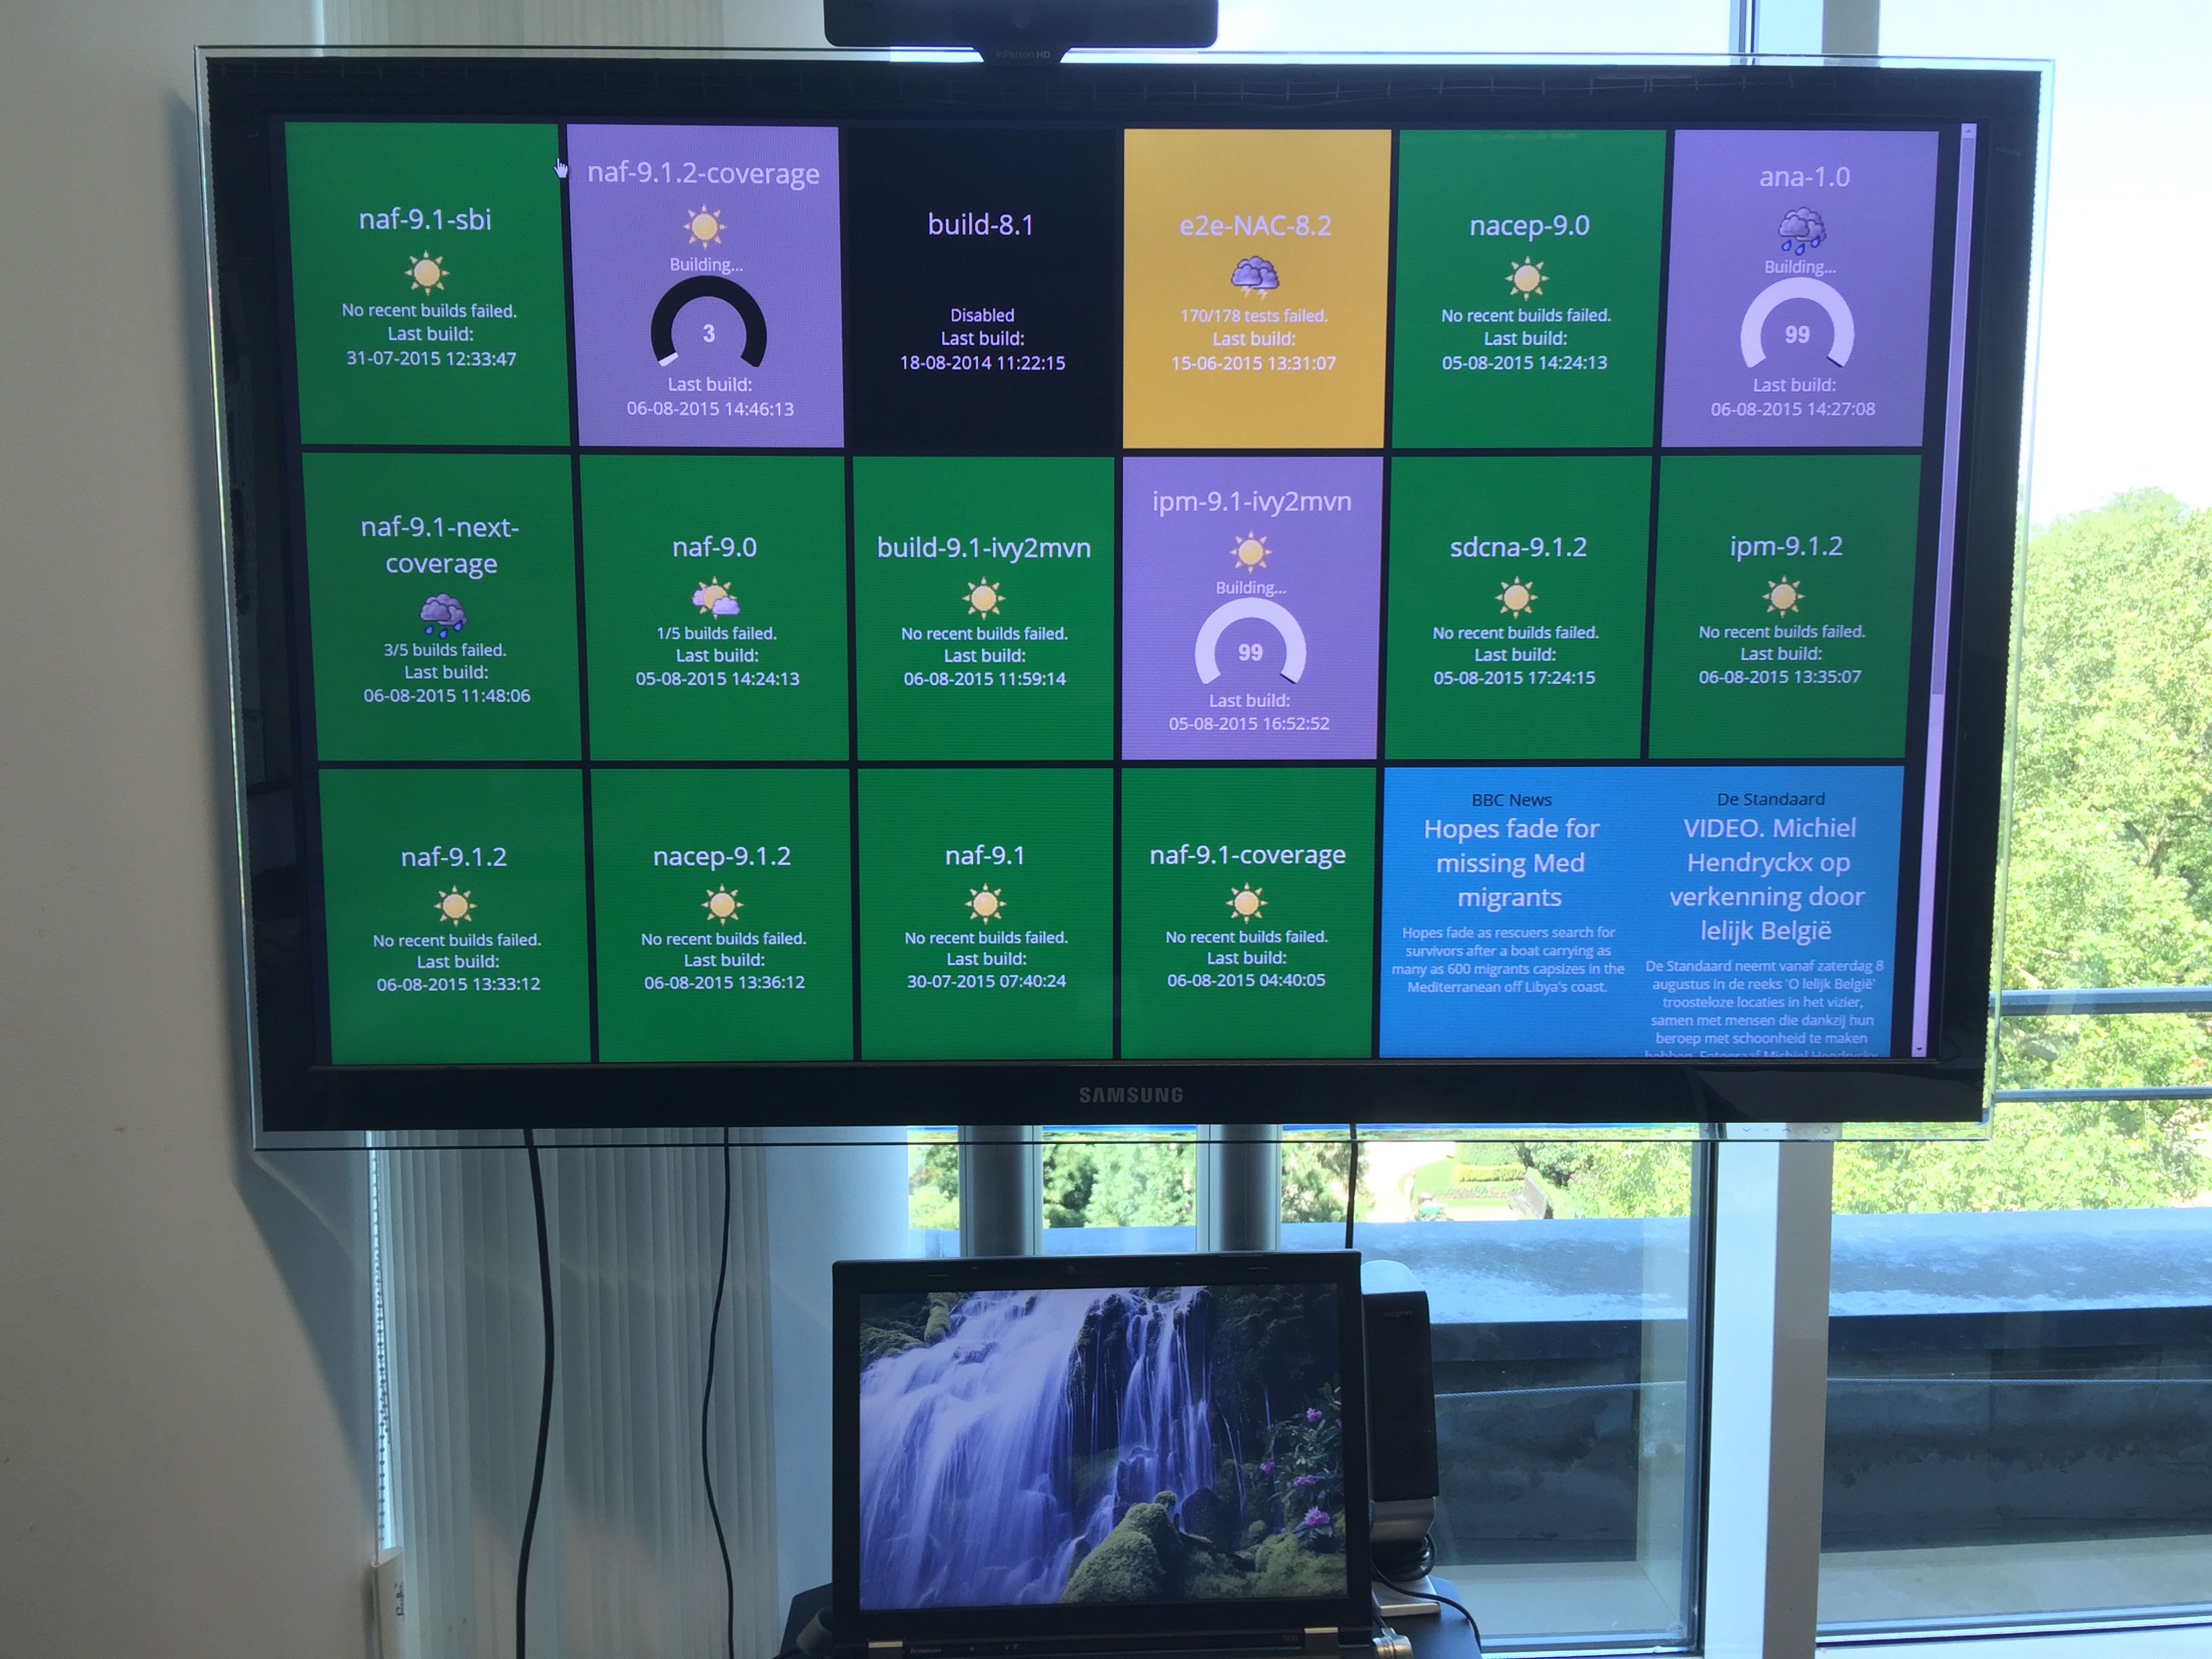
\includegraphics[width=60mm]{dashboardresult.jpg}
\caption{Finale dashboard op televisie.}
\label{dash_4}
\end{minipage}
\end{figure}

\begin{figure}[ht!]
\centering
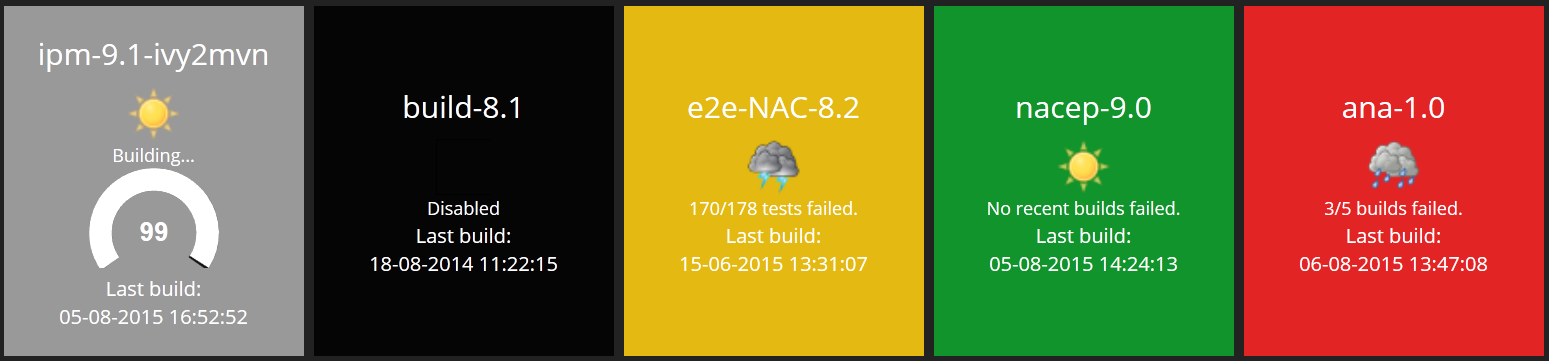
\includegraphics[width=90mm]{dashboard_screenshot5.png}
\caption{Gedetailleerd overzicht van de finale versie van het dashboard.} 
\label{dash_5}
\end{figure}

\subsection{Initiatieven voor stagiairs}
\label{interns}
Alcatel-Lucent organiseerde in de zomer van 2015 een initiatief om alle stagiairs met elkaar in contact te brengen tijdens speciale info-events en \textit{meetings}. Op deze manier konden stagiairs van verschillende afdelingen met elkaar bespreken hoe de stage op hun afdeling verliep en zo ervaringen met elkaar uitwisselen. Er zijn verschillende contactmomenten georganiseerd, meestal tijdens de middagpauze. Er waren verschillende bijeenkomsten, waaronder samen lunchen om kennis te maken en een gesprek met Joeri Veldeman, begonnen als doctor in de \textit{electrical engineering} bij Alcatel-Lucent en nu hoofd van de afdeling van \textit{human resources}. Zijn ongewone carri\`erepad werd besproken en hij er werd informeel gesproken over de verdere studietrajecten van de stagiairs.
Verder is er een infosessie geweest over ALU Labs, waarin enkele van de zaken aan bod kwamen waarin Alcatel-Lucent investeert en onderzoek bij uitvoert. Er was ook een infosessie over \textit{fixed networks}, waarbij uitleg gegeven werd over wat het team in Antwerpen allemaal verwezenlijkt en waarbij een bezoek gebracht werd aan een van de labo's.\\
Dit alles maakte dat de stage niet alleen een verrijking van kennis binnen de afdeling werd, maar ook daarbuiten, waarbij contact met andere studenten gelegd werd.

\section{Relatie stage en opleiding}
\label{relatie}
De stage-opdracht bestond uit het maken van een dashboard zodat de \textit{build} status van de verschillende onderdelen van projecten overzichtelijk getoond kunnen worden. Binnen deze stage werd ik dankzij de goede begeleiding van Bart bovendien ook betrokken bij alle bijeenkomsten met het team, om zo te ervaren hoe het er in een werkomgeving aan toe gaat. Op deze manier zijn er extra facetten aan bod gekomen die ook tijdens de opleiding Informatica aan bod zijn gekomen. Hieronder is de relatie tussen de stage en de opleiding beschreven.

\begin{description}
\item[Informatica werktuigen]
Tijdens de lessen van Informatica werktuigen zijn Ruby, Linux en LaTeX aan bod gekomen. Ruby bleek nuttig om de (Embedded) Ruby voor het dashboard te schrijven, waar de kennis van Linux ervoor zorgde dat werken met Linux in het algemeen vlot ging, gezien het dashboard in Linux is ontwikkeld. LaTeX is gebruikt om de literatuurstudie te maken en het verslag op te stellen.
Doordat er in de bachelor Informatica al een heel aantal programmeertalen gezien werden, was het aanleren van andere (opmaak)talen veel makkelijker.

\item[Objectgericht Programmeren]
Voor het maken van het dashboard werd er gebruik gemaakt van een bestaand \textit{framework}, maar er is nog een groot deel code bijgeschreven. Omdat er gebruik gemaakt werd van bestaande code, werd het duidelijk hoe belangrijk goede documentatie is, gezien de bestaande code op zich nauwelijks/niet gedocumenteerd was, wat het begrijpen van de code moeilijker maakte. Het schrijven van (goede) documentatie is iets waar tijdens de lessen van Objectgericht Programmeren de nadruk op lag. De documentatie op de websites van het framework en de plugins was vaak onvolledig, wat het opzoeken van functionaliteiten moeilijker maakte. Om die redenen is er tijdens het ontwikkelen van het dashboard eigen documentatie geschreven. Om hergebruik en aanpassing te vergemakkelijken, zijn er handleidingen geschreven op de wiki van Alcatel-Lucent.

\item[Software-ontwerp]
Op de afdeling NA-C in Antwerpen werkt men volgens de \textit{agile}-methode, waar \textit{scrum} een onderdeel van is, met elke dag \textit{stand-up meetings} en tweewekelijkse sprints. Dit is iets wat in de lessen van Software-ontwerp aan bod is gekomen, waarvan tijdens de stage bleek dat het echt zijn nut heeft. De korte sprints en regelmatige \textit{reviews} zorgen ervoor dat problemen niet te lang kunnen blijven bestaan en omdat er bijna dagelijks gepraat wordt over wie waarmee bezig is, kunnen mensen elkaar vlot helpen en weet iedereen wie waarmee bezig is.\\
Een tweede aspect uit Software-ontwerp dat tijdens de stage aan bod kwam is \textit{pair-programming}. De stage-opdracht was onafhankelijk van de projecten bij NA-C, maar bij vragen bij het ontwikkelen van het dashboard is er wel aan \textit{pair-programming} gedaan met de werknemers van NA-C. \\
Het dashboard dat ontwikkeld moest worden mocht geen kant-en-klaar dashboard zijn waar zelf info aan toegevoegd werd, maar \'e\'en waarbij moest nagedacht worden over het ontwerp en de implementatie van de code om het dashboard te realiseren. Dit werd behandeld in de lessen van Software-ontwerp.

\item[P\&O]
Voor de stage-opdracht werd een eigen \textit{scrum}project voorzien, waarbij ook over sprints ge\"itereerd werd. Die manier van werken is vergelijkbaar met deze tijdens de P\&O-sessies van de bachelorproef, waarbij we om de paar weken een bepaalde functionaliteit van de robot moesten kunnen demonstreren.

\item[Software-Ontwerp en P\&O]

Waar versiecontrole tijdens het project van Software-ontwerp werd aangeraden, maar niet verplicht was, werd het bij P\&O wel verplicht. Hiervan is gebruik gemaakt bij het ontwikkelen van het dashboard (zij het aan de late kant, zie de kritische reflectie van de competenties in Sectie \ref{reflectie}) tijdens een groot deel van de stage.

\item[Wetenschapscommunicatie en P\&O]

Het schrijven van (wetenschappelijke) verslagen was een belangrijk onderdeel bij de vakken Wetenschapscommunicatie en P\&O, wat hielp bij het schrijven van de literatuurstudie en het stageverslag.
\end{description}
Binnen de opleiding Informatica wordt er altijd gewerkt in kleine groepjes, meestal van twee mensen, maximaal in groepen van zes mensen. Op de afdeling NA-C werkt men in een team van ongeveer 10 mensen, wat het managen\todo{ander woord?} van het team nog moeilijker maakt dan bij een groep van slechts enkele mensen. Toch is er getoond dat dit perfect mogelijk is indien je de juiste \textit{tools} gebruikt (bij NA-C maakt men gebruik van Confluence en JIRA) en indien er goed gecommuniceerd wordt.

\section{Kritische reflectie competenties}
\label{reflectie}
Het originele document met competenties die ik wenste te verbeteren is te vinden in Appendix \ref{competenties}.
\begin{itemize}
\item Technische competenties die ik hoopte te verbeteren:
\begin{description}

\item[Bijleren over \textit{version control}] Er wordt op de afdeling NA-C gewerkt met Git, waar ik ook tijdens mijn opleiding al mee in aanraking ben gekomen. Tijdens de eerste fase van de ontwikkeling van het dashboard heb ik geen gebruik gemaakt van Git, hoewel dit zeker nuttig geweest zou zijn. Eens de eerste versie van het dashboard klaar was, is er gebruik gemaakt van Git\footnote{De code is te vinden op https://github.com/HelenaCat/jenkins-dashboard}, maar dit had dus veel eerder moeten gebeuren. Er is gebruik van gemaakt bij het toevoegen van documentatie en bij het maken van veranderingen tijdens de derde sprint.\\
Ondanks het te laat beginnen gebruiken van versiecontrole, zijn mijn competenties hierrond wel verbeterd, gezien ik Git nu ook via de \textit{command line} in Linux heb leren gebruiken en niet alleen in de grafische \textit{user interface} op Windows. 

\item[Leren werken met Jenkins] Op de afdeling NA-C wordt gewerkt met het \textit{continuous integration} systeem Jenkins, dat \textit{builds} automatisch \textit{runt} nadat er een nieuwe versie van de software \textit{gecommit} is. Tijdens de stage was het duidelijk hoe nuttig dit is: er werd op een gegeven moment een fout gemaakt, die ook nog eens onvoldoende getest bleek, maar men heeft die heel snel ontdekt en binnen de 2 dagen kunnen oplossen. Moest er gewacht zijn met \textit{mergen} tot vlak voor de \textit{release}, was men waarschijnlijk veel meer problemen tegengekomen. \textit{Continuous integration} is vooral handig indien er in groep wordt gewerkt, het was dus van pas gekomen tijdens P\&O of Software-Ontwerp. \todo{dat laatste weglaten?}

\item[Mij inwerken in een reeds lopend project] Ik moest niet meewerken aan de code van het NA-C team zelf, maar heb mij wel moeten inwerken in de code van het dashboard. Zoals hierboven vermeld, was dit niet altijd makkelijk, maar het heeft er wel voor gezorgd dat ik enorm veel heb bijgeleerd, net omdat ik heel veel zelf moest uitzoeken. Eens de eerste versie van het dashboard klaar was, kende ik de code enorm goed, dus nieuwe veranderingen konden zeer snel ge\"implementeerd worden.
\end{description}

\item Persoonlijke competenties die ik hoopte te verbeteren:
\begin{description}
\item[Leren werken in grote teams] In het NA-C team in Antwerpen werken er een tiental mensen, in Bangalor en Chennai zijn er teams van gelijkaardige grootte. Doordat er dagelijks een \textit{standup meeting} was met de mensen van het team in Antwerpen, was iedereen goed op de hoogte van wie wat deed en doordat men met sprints van twee weken werkte, kwamen problemen snel boven. Dit is iets dat ik zeker meeneem naar projecten in de toekomst toe, ik heb ervaren hoe al deze zaken kunnen helpen in het beter doen verlopen van een project.
\item[Plannen op lange termijn] Aan het begin van de stage werd me meteen gezegd dat ik redelijk vrij gelaten ging worden in mijn planning, maar er werd wel gevraagd om er een op te stellen, zodat ik ook in sprints kon werken. Ik heb zelf voorstellen mogen doen en aan mijn eigen tempo (maar toch binnen de termijnen van de sprints) kunnen werken. Als er grote dingen te doen stonden, plande ik daar altijd genoeg tijd voor in, zodat ik uiteindelijk ``te vroeg" klaar was en aan verbeteringen kon werken. Dit is een van de competenties die ik zowel in het tweede semester van mijn laatste bachelorjaar heb aangescherpt, als nu op de stage, dankzij de goede begeleiding van Bart.  
\end{description}
\end{itemize}

\section{Conclusies}
\label{conclusies}
Het doel van de stage was om Jenkins-\textit{awareness} te cre\"eren door het maken van een dashboard waarop het overzicht van de \textit{build} statussen duidelijk te zien zijn. De eerste taak bestond uit het maken van een literatuurstudie om een idee te vormen van hoe een goed dashboard eruit moet zien. Ook werd er gekeken welke \textit{frameworks} er aanwezig zijn om dashboards te ontwikkelen. De literatuurstudie heeft ervoor gezorgd dat er duidelijke doelstellingen voor de layout van het dashboard voor ogen gesteld konden worden, waarbij de voorstellen die uit de enqu\^ete kwamen hielpen om extra zaken toe te voegen die belangrijk waren voor het team. Vervolgens is het dashboard ontwikkeld en zijn er extra elementen toegevoegd of veranderd na het uitvoeren van een tweede enqu\^ete. De doelstellingen die voor de stage werden gesteld zijn behaald, gezien er aan het einde van de stage een werkend dashboard kon voorgelegd worden die voldeed aan de vereisten die zijn opgemaakt in de literatuurstudie. \\ 
Doordat de begeleiding tijdens de stage erg goed was en omdat de medewerkers van het NA-C team in Antwerpen regelmatig hun mening gaven, is het dashboard met de gevraagde vereisten gerealiseerd kunnen worden.
De stage was enorm leerzaam dankzij de enorme betrokkenheid die gevraagd werd bij alles wat het NA-C team in Antwerpen deed. Hoewel de stage-opdracht los stond van het werk op de afdeling, werden \textit{meetings} bijgewoond om te tonen hoe alles in zijn werk gaat. Het bijwonen van sprint \textit{meetings} toonde hoe de \textit{agile} werkmethode zijn nut heeft en hoe goede communicatie essenti\"eel is voor het slagen van projecten, ook het project van de stage.
De stage heeft enorm veel geleerd over het samenwerken in groepen en over het (grotendeels) zelfstandig uitwerken van projecten. Doordat het project individueel werd gerealiseerd, werden alle aspecten zelfstandig uitgewerkt: er moest in bestaande code ingewerkt worden en de doelen voor het project moesten ook individueel behaald worden. Deze zaken gebeuren tijdens de opleiding Informatica meestal in groep, waardoor het uitwerken van projecten anders ervaren wordt dan wanneer ze zelfstandig worden gemaakt.\\
Er kan besloten worden dat de stage een meerwaarde was, gezien er nieuwe (opmaak)talen geleerd werden, competenties aangescherpt zijn (werken met Git, werken in Linux,\ldots), er getoond werd hoe grote groepen goed kunnen samenwerken, ook vanop verschillende locaties, en ten slotte hoe projecten onder begeleiding zelfstandig uitgewerkt kunnen worden. De vaardigheden die hier zijn aangeleerd en verscherpt kunnen zeker meegenomen worden in het verdere traject van de opleiding.
\todo{nalezen \& verbeteren}

\section{Besluit}
\label{besluit}
De stage ging voor 6 weken door bij Alcatel-Lucent in Antwerpen op de afdeling Network-Analyzer Copper. De opdracht was het ontwerpen van een dashboard om de \textit{build} status van het \textit{continuous integration} systeem Jenkins te tonen. Het ontwikkelen van het dashboard is gebeurd gebruik makende van de \textit{agile} werkmethode, waarbij in sprints van twee weken gewerkt werd.\\
Het dashboard is succesvol gemaakt binnen de opgelegde tijd met behulp van Dashing, draaiende op een Linux server.\\
Tijdens de stage is gebruik gemaakt van onder andere Javascript, JQuery, HTML en (S)CSS. Mijn kennis van Ruby en Linux kwam hierbij ook van pas.\\
Onder de goede begeleiding van Bart en dankzij de hulp van de mensen bij NA-C in Antwerpen zijn de opgelegde doelen grotendeels zelfstandig uitgewerkt en werd er getoond hoe werken in grote teams in een bedrijf verloopt.

\clearpage

\begin{thebibliography}{11} 

\bibitem{dashing} Daniel Beauchamp, Serena Ngai, Wesley Ellis, David Underwood (2015). \emph{Dashing The exceptionally handsome dashboard framework}. [09/07/2015, uitgever: http://dashing.io/].

\bibitem{learndashing} Larry Cai (05/05/2014). \emph{Learn Dashing Widget in 90 minutes}. [21/07/2015, uitgever: http://www.slideshare.net/larrycai/learn-dashing-widget-in-90-minutes].

\bibitem{huawei} Julia Fioretti (07/05/2015). \emph{Huawei undeterred by Nokia's Alcatel-Lucent deal}. [07/07/2015, uitgever: http://www.reuters.com/article/2015/05/07/us-huawei-outlook-ceo-idUSKBN0NS23P20150507].

\bibitem{fowler} Martin Fowler (13/12/2005). \emph{The New Methodology}. [08/09/2015, uitgever: http://martinfowler.com/articles/newMethodology.html].

\bibitem{jenkins}  Kohsuke Kawaguchi, Larry Shatzer (28/07/2015). \emph{Meet Jenkins}. [06/07/2015, uitgever: https://wiki.jenkins-ci.org/display/JENKINS/Meet+Jenkins].

\bibitem{batman} Nick Small (2013). \emph{Meet your new favorite JavaScript superhero}. [22/07/2015, uitgever: http://batmanjs.org/].

\bibitem{widgets} Matt Snider (28/08/2015). \emph{Additional Widgets}. [05/08/2015, uitgever: https://github.com/Shopify/dashing/wiki/Additional-Widgets ].

\bibitem{agile} Geen auteur opgegeven (08/09/2015). \emph{Agile software development}. [05/08/2015, uitgever: https://en.wikipedia.org/wiki/Agile\_software\_development].

\bibitem{history} Geen auteur opgegeven (2015). \emph{Alcatel-Lucent History}. [06/07/2015, uitgever: https://www.alcatel-lucent.com/about/history].

\bibitem{operations} Geen auteur opgegeven (2015). \emph{How we operate}. [06/07/2015, uitgever: https://www.alcatel-lucent.com/about/operations].

\bibitem{codecademy} Geen auteur opgegeven (2015). \emph{Learn to code interactively, for free}. [21/07/2015, uitgever: https://www.codecademy.com/].

\bibitem{markets} Geen auteur opgegeven (2015). \emph{Our markets}. [08/09/2015, uitgever: https://www.alcatel-lucent.com/about/markets].

\bibitem{scrumrugby} Geen auteur opgegeven (07/09/2015). \emph{Scrum (rugby)}. [05/08/2015, uitgever: https://en.wikipedia.org/wiki/Scrum\_\%28rugby\%29].

\bibitem{scrumsw} Geen auteur opgegeven (01/09/2015). \emph{Scrum (software development)}. [05/08/2015, uitgever: https://en.wikipedia.org/wiki/Scrum\_\%28software\_development\%29].

\bibitem{jira} Geen auteur opgegeven (2015). \emph{The flexible and scalable issue tracker for software teams}. [06/07/2015, uitgever: https://www.atlassian.com/software/jira].

\bibitem{userstory} Geen auteur opgegeven (05/09/2015). \emph{User story}. [09/07/2015, uitgever: https://en.wikipedia.org/wiki/User\_story].

\bibitem{waterfall} Geen auteur opgegeven (31/08/2015). \emph{Waterfall model}. [05/08/2015, uitgever: https://en.wikipedia.org/wiki/Waterfall\_model].


\iffalse

Auteur(s) (datum van laatste update). \textit{Titel van het document}. [raadplegingsdatum, uitgever: URL]. 


https://www.alcatel-lucent.com/about/history
https://www.alcatel-lucent.com/about/operations
http://www.reuters.com/article/2015/05/07/us-huawei-outlook-ceo-idUSKBN0NS23P20150507
https://en.wikipedia.org/wiki/Waterfall_model
https://en.wikipedia.org/wiki/Agile_software_development
http://martinfowler.com/articles/newMethodology.html
https://en.wikipedia.org/wiki/Scrum_%28software_development%29
https://en.wikipedia.org/wiki/Scrum_%28rugby%29
https://en.wikipedia.org/wiki/User_story 
https://www.atlassian.com/software/jira
https://jenkins-ci.org/
http://dashing.io/
http://batmanjs.org/
https://www.codecademy.com/
https://github.com/Shopify/dashing/wiki/Additional-Widgets 
http://www.slideshare.net/larrycai/learn-dashing-widget-in-90-minutes
\fi


\end{thebibliography}

\clearpage

\begin{appendices}
\section{Literatuurstudie}
\label{lit_study}


\paragraph{General}
A dashboard is a tool to quickly show information at a glance. Its purpose is to have the ``reader" gather information without having to look things up; everything should be clear by having a quick look at the dashboard. At Alcatel-Lucent, they make use of the Jenkins dashboard, but it doesn't comply with the given description: in order to see what builds failed/succeeded, you need to find the build you're looking for and then check its status. It is clear from the -lack of- its use that this way of displaying the information does not suffice, since the TV dashboard is not/barely used but every employer looks up the dashboard on their own PC every once in a while. \\

The purpose of this literature study is to create Jenkins awareness, so the developers can take a look at the TV dashboard a few times a day and have them see how the project is proceeding.\\
One of the most important things is that the information displayed on the dashboard can be easily interpreted. This means that you don't want a cluttered dashboard with too much information so it becomes unclear.
Stephen Few has written an excellent article on the topic, with the main conclusions being:
\begin{itemize}
\item don't show too much information,
\item keep the information simple,
\item colors should be used sparingly or they will mean nothing at all,
\item visuals should be useful; not overwhelming or distracting and
\item the information represented should be accurate, so you should make sure the information is displayed correctly and with enough context.
\end{itemize}

This last remark is also made by Matthew Skelton\footnote{(Skelton, 2013, http://blog.matthewskelton.net/2013/03/11/what-makes-an-effective-build-and-deployment-radiator-screen/)}, who shows that if you only show the failed builds, people will start to ignore the 'alarm signals' the dashboard displays and perform less well compared to when a context is shown, also showing the successful builds. \\  
Few’s theory is backed up by the people at Geckoboard, who have made a blog consisting of 6 parts, referencing to Few, but also adding some rules of thumb\footnote{(Smith, 2012, https://www.geckoboard.com/blog/building-great-dashboards-6-golden-rules-to-successful-dashboard-design/)}. Every article listed in the appendix refers to Few’s article and some make additional remarks. 
One of them is that it’s very important to keep your audience in mind, the board of directors will want to see different metrics represented in the dashboard than, say, the people of human resources. 
In the case of software developers, they’ll want to see metrics about the build status of the different jobs. Related to this is that not every dashboard will need the same layout and look. \\
In the case of the Jenkins dashboard, charts won’t tell you much, since it doesn’t really tell anything about the status of the last build. Below, the example of the Jenkins dashboard is further explained and a proposal is made that conforms to the guidelines of a good dashboard.

\paragraph{Improving the Jenkins dashboard}
The Jenkins dashboard, as seen in Figure \ref{jenkins}, displays a list of the builds of a project, together with a colored dot and a ``weather report". The dot displays information about the last build, the color indicating whether it failed or succeeded and a flashing dot meaning the build is still in progress. 
The color of the dot at that time then refers to the last finished build.
The weather report tells you something about the stability of the builds. If the weather looks good, then the build is stable. The worse the weather gets, the less stable the build is. This way, you get an overall view about the stability of the different build jobs.

\begin{figure}[ht!]
\centering
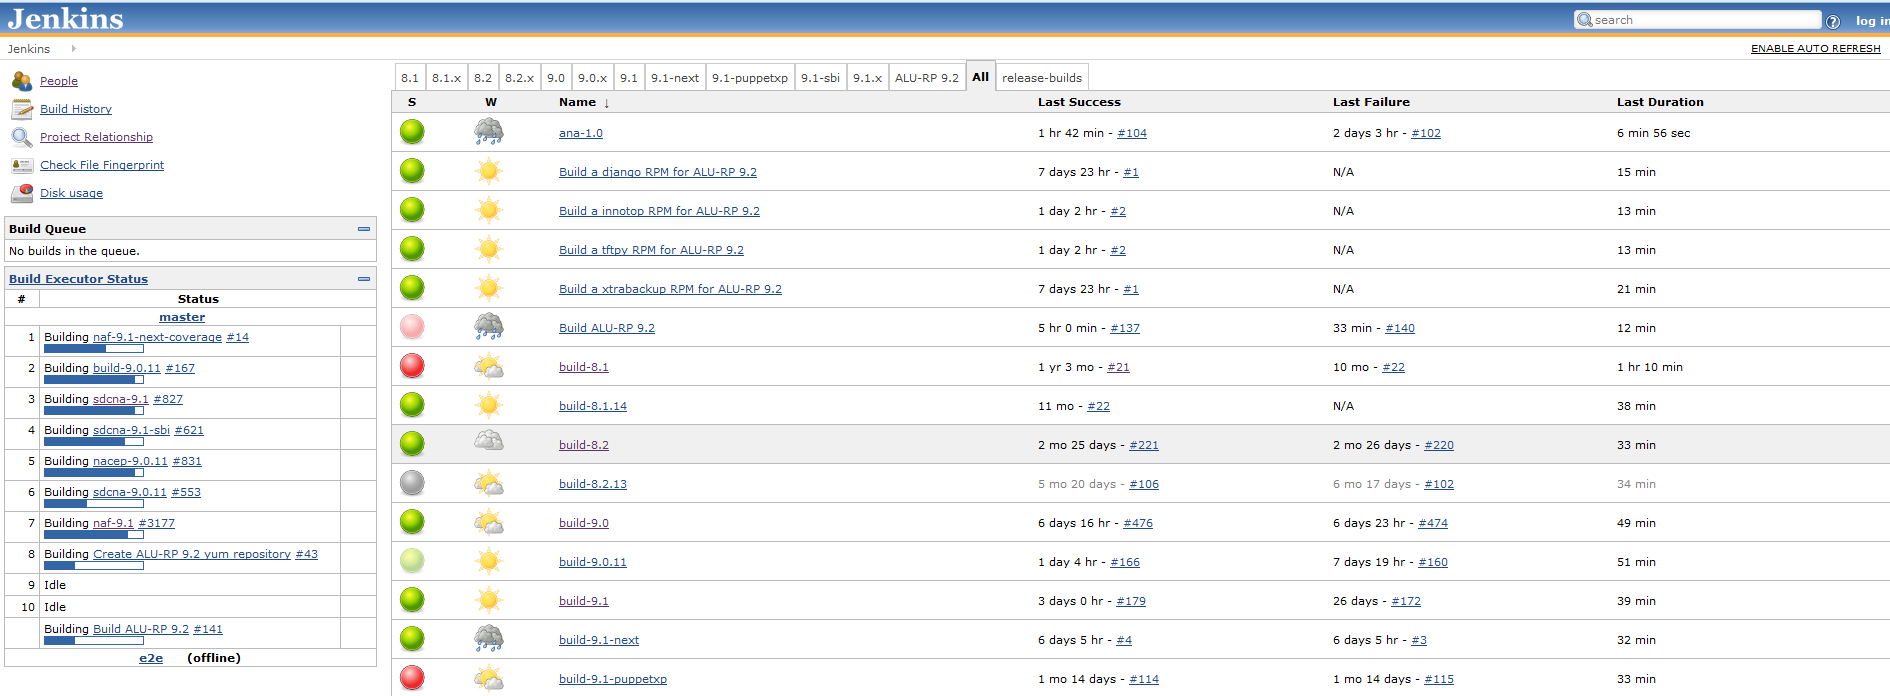
\includegraphics[width=90mm]{CaptureJenkins.png}
\caption{The Jenkins dashboard.} 
\label{jenkins}
\end{figure}
 
These two things give you a fairly good overview, but the downside of the dashboard is that you have to be right in front of the screen to see what job the colored dot and the weather report are referring to. 
The details of the build job are in plain text, so if you want to project it on a TV screen, people will have a hard time knowing what builds are doing well and which ones aren't.
There are plug-ins available that show a dashboard, but they none of them comply with the most important rules described above: they're either too crowded or use too much color, distracting the viewer from what's really important.

\begin{figure}
\centering
\begin{minipage}{0.45\textwidth}
\centering
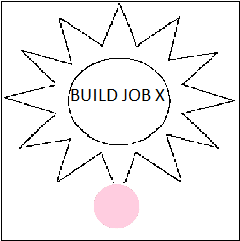
\includegraphics[width=60mm]{prop1.png}
\caption{Proposal 1.}
\label{prop1}
\end{minipage}\hfill
\begin{minipage}{0.45\textwidth}
\centering
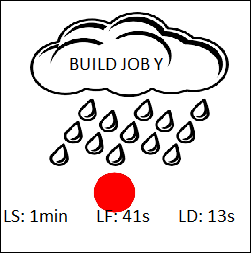
\includegraphics[width=60mm]{prop2.png}
\caption{Proposal 2.}
\label{prop2}
\end{minipage}
\end{figure}
  
The proposed images, as seen in Figure \ref{prop1} and \ref{prop2} comply with the design problems to be avoided as proposed by Stephen Few:
\begin{itemize}
\item Too much complexity
\item Too many alert conditions
\item Alerts that cannot be differentiated
\item Overwhelming visuals
\item Distracting visuals
\item Inappropriate visual salience
\item Mismatch between information and its visual representation
\item Indirect expression of measures
\item Not enough context
\end{itemize}
The images show the build stability together with the success or failure of the last build and show the name of the build clearly. It's also possible to add a timestamp of when the last success and failure were and the last duration at the bottom of the tiles, as shown in Figure \ref{prop2}. If you have color blind people in your team (as Few pointed out might happen), you could replace the green dot by a very light red dot, indicating it doesn't need attention, as shown in Figure \ref{prop1}.
This could be realized using existing Jenkins plug-ins and changing them. The Radiator View\footnote{(Skelton, 2013, http://blog.matthewskelton.net/2013/03/11/what-makes-an-effective-build-and-deployment-radiator-screen/)} seems like a good basis.
An alternative could be to implement already existing software like Dashing\footnote{(Beauchamp, Ngai, Ellis, Underwood, 2015, dashing.io)}, which provides the tools to generate dashboards very easily. Instead of showing the weather as proposed, color codes may be used for the tile backgrounds, either representing the status of the last build or the status of the past builds. A combination is also possible where the color represents the status of the last build and an opaque weather report image as the background. An example is given in Figure \ref{dash}:

\begin{figure}[ht!]
\centering
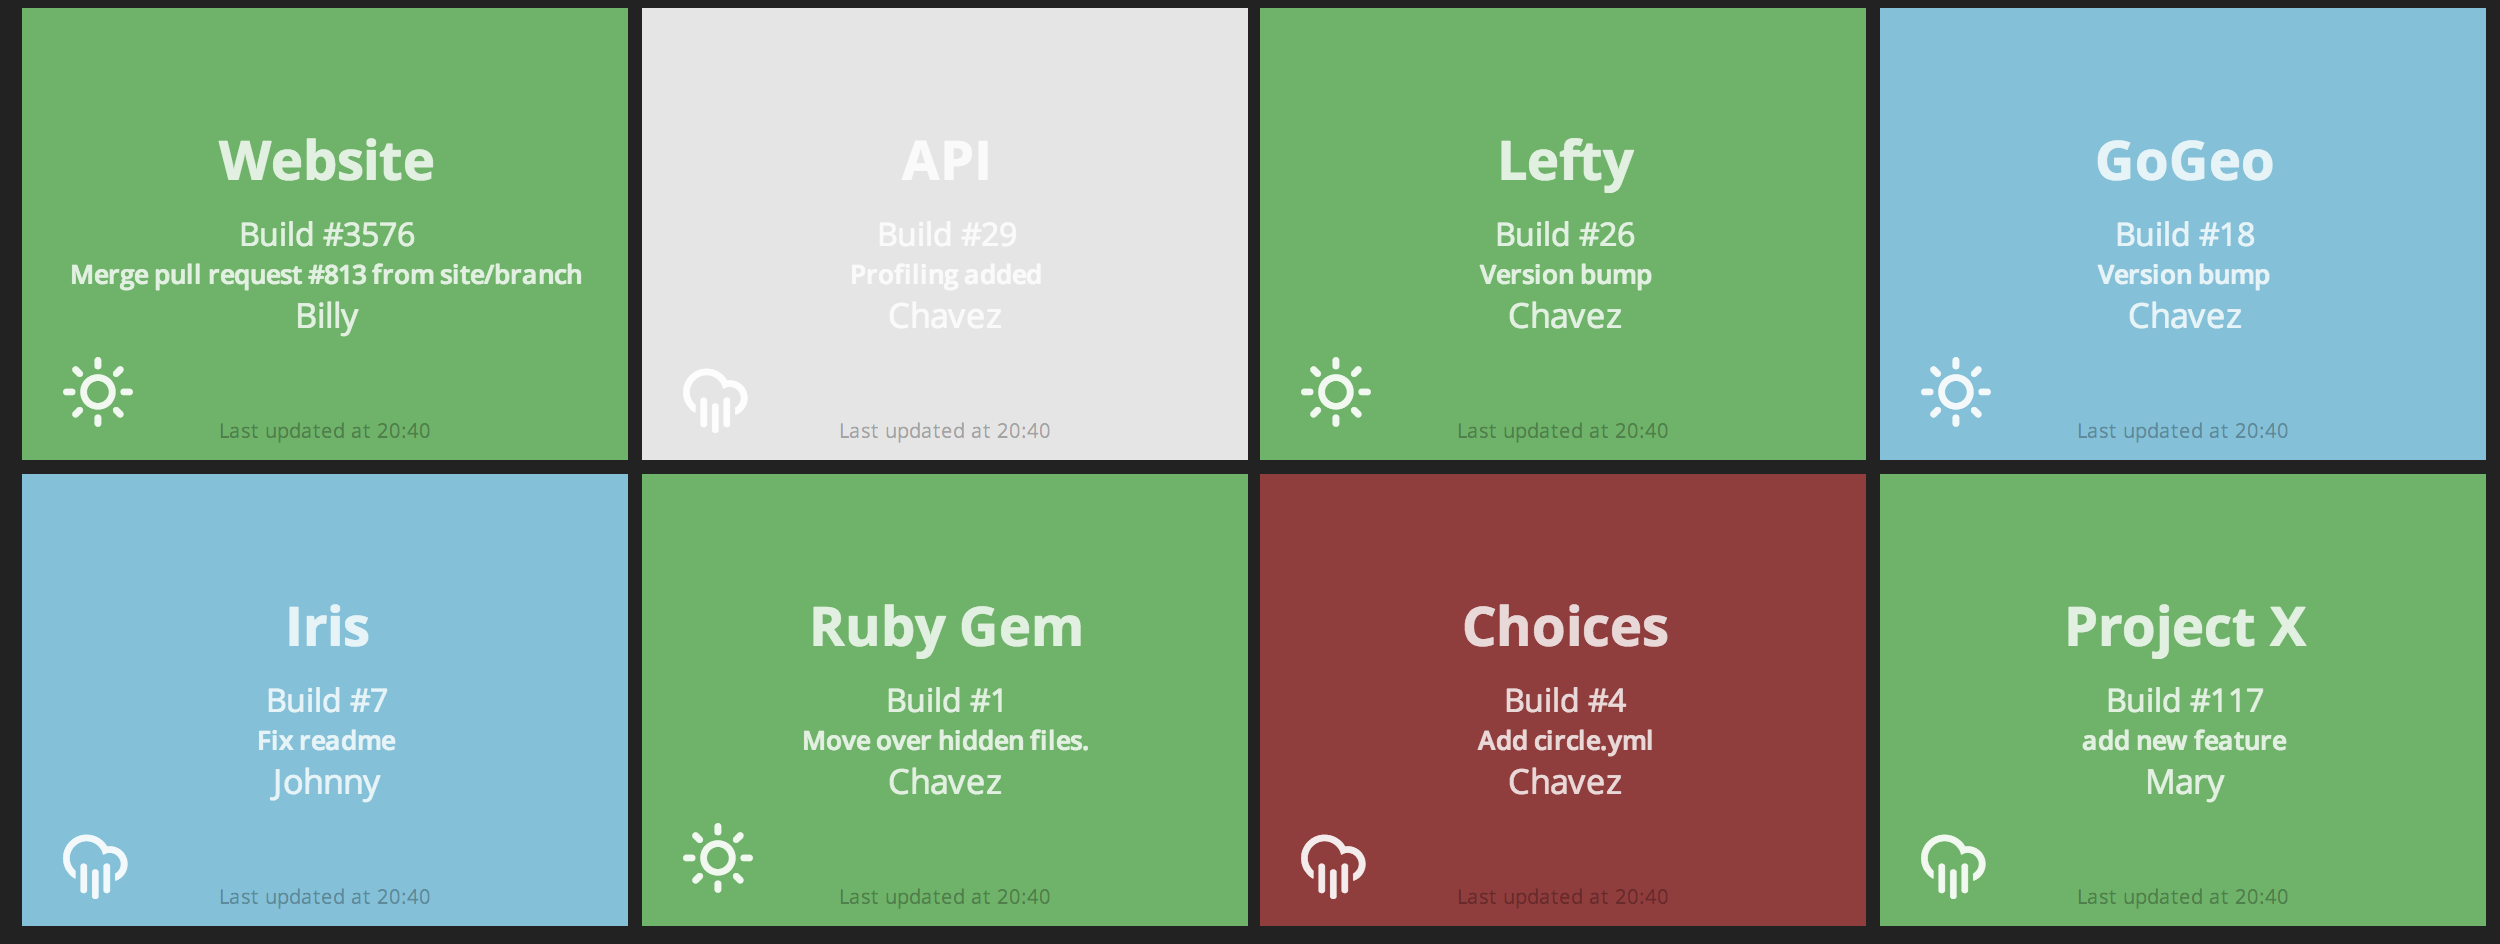
\includegraphics[width=90mm]{dashboard-prop.png}
\caption{Example dashboard for Jenkins.} 
\label{dash}
\end{figure} 
 
The colors aren’t too overwhelming and they’re meaningful, since people are used to the colored dots in the Jenkins dashboard. 
A third, less tile-oriented dashboard is Team Dashboard\footnote{(Dietz, 2013, http://fdietz.github.io/team\_dashboard/)}. It also supports Jenkins plug-ins.


\begin{thebibliography}{11} 

\bibitem{gemignani} Zach Gemignani. \emph{A Dashboard Alerts Checklist.} [09/07/2015, published at: http://www.juiceanalytics.com/writing/dashboard-alerts-checklist/]

\bibitem{few} Stephen Few (2007). \emph{Dashboard Design For Real-Time Situation Awareness.} [09/07/2015, published at: http://www.perceptualedge.com/articles/Whitepapers/Dashboard\_Design.pdf]

\bibitem{skelton} Matthew Skelton. \emph{What Makes an Effective Build and Deployment Radiator Screen?.} [09/07/2015, published at: http://blog.matthewskelton.net/2013/03/11/what-makes-an-effective-build-and-deployment-radiator-screen/]

\bibitem{smith} Nick Smith. \emph{Designing and Building Great Dashboards - 6 Golden Rules to Successful Dashboard Design.} [09/07/2015, published at: https://www.geckoboard.com/blog/building-great-dashboards-6-golden-rules-to-successful-dashboard-design/]

\bibitem{juice} No author specified. \emph{A Guide to Creating Dashboards People Love to Use.} [10/07/2015, published at: http://www.cpoc.org/assets/Data/guide\_to\_dashboard\_design1.pdf]

Images:

\bibitem{sun} \emph{Sun.} [http://azcoloring.com/coloring-page/112445]

\bibitem{rain} \emph{Rain cloud.} [http://www.clipartpanda.com/categories/animated-rain-clouds]

\bibitem{red_dot} \emph{Red dot.} [http://www.thepointless.com/reddot]

\bibitem{pink_dot} \emph{Pink dot.} [http://www.create-a-mural.com/dry-erase-11-soft-pink-dot-decal.html]

\bibitem{dashboard} \emph{Example dashboard.}  [https://camo.githubusercontent.com/
1509a366bd27fad24ba09c45793308a85bcbf8bf/687474703a2f2f662e636c2e6c792f6974656d732
f336330743076335a31313145306f3436333033322f53637265656e25323053686f742532303230313
32d31302d30332532306174253230382e34362e3437253230504d2e706e67]

\end{thebibliography}
\clearpage

\section{Enqu\^ete 1}
\label{enquete1}
\paragraph{Enqu\^ete}
De enqu\^ete bestond uit een reeks voorbeeldtegels met bepaalde kenmerken (zie Figuur \ref{proposals}) die ook in de enqu\^ete zelf uitgelegd werden (het deel boven ``Preferences"). De enqu\^ete bestond uit volgende vragen, met ruimte om commentaar te voorzien:\\

\begin{minipage}{1.1 \textwidth}
\begin{quote}
``Hello" == name of build
\begin{enumerate}
\item No progress meter for the currently running build. Background color indicating the success/failure of the last completed build, big weather report about the last builds.
\item Small meter showing the progress of the currently running build, weather report at the bottom, background color indicating success/failure of last completed build.
\item Small meter with weather report on top, background color indicating success/failure.
\item Circular meter with weather report on top, background color indicating success/failure of last build.
\end{enumerate}
Preferences (circle the preference)
\begin{itemize}
\item Meter/no meter; in case of meter:
\begin{itemize}
\item Large/small
\item On top/at bottom
\item Circular/dashboard-like
\end{itemize}
\item Weather report/no weather report
\item Background color/no background color (colored dot is better)
\end{itemize}
\end{quote}

\end{minipage}

\begin{figure}[ht!]
\centering
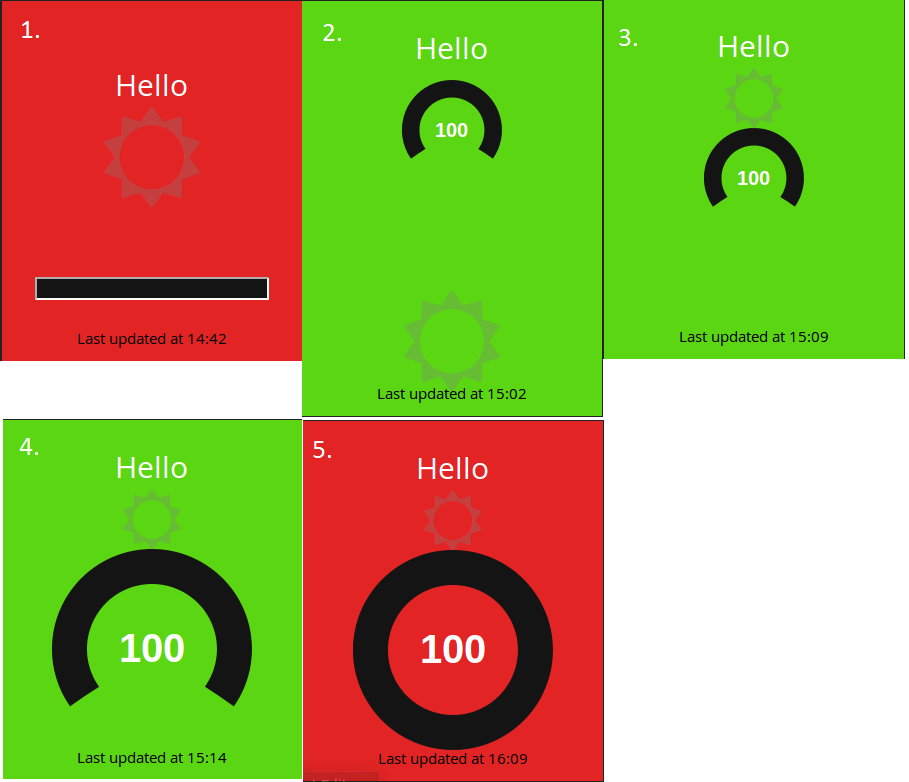
\includegraphics[width=90mm]{proposals.png}
\caption{Voorbeeldwidgets.} 
\label{proposals}
\end{figure} 

\paragraph{Resultaten}
De resultaten zijn te zien in Tabel \ref{results}. Let op, niet iedereen heeft op elk onderdeel geantwoord, daarom zijn er niet op elke vraag 9 antwoorden.

\begin{table}[h!]
\centering
\begin{tabular}{|c|c|c|}
\hline                         										
		 			&	Yes 		&	No		\\	\hline	\hline
Meter				&	8			&	0		\\	\hline
-Large				&	4			&	4		\\	\hline
-On top				&	1			&	6		\\	\hline	
-Circular			&	3			&	5		\\	\hline
Weather report		&	8			&	1		\\	\hline
Background color	&	9			&	0		\\	\hline
\end{tabular}
\caption{Resultaten van de eerste enqu\^ete}
\label{results}
\end{table}

Bijkomende opmerkingen zijn de volgende:
\begin{itemize}
\item ``Would combine 1 and 3. Big weather report with small meter at the bottom"
\item ``It would be nice if we can show the failure count for failure builds"
\item ``I would replace 'last updated' with latest finished build and building since (if in progress). Only show meter when busy building"
\item ``Overview of last builds = list or circle with \% of failed/success"
\item ``I'd put more visibility for the weather report/more important than current build progress. Maybe also add the date of the last build/number of test or failing tests?"
\end{itemize}

\clearpage

\section{Powerpoint presentatie dashboard sprint 2}
\label{ppt}

\begin{figure}[!h]
\centering
\begin{minipage}{0.45\textwidth}
\centering

\includegraphics[width=60mm]{ppt1.pdf}
\label{standup}
\end{minipage}\hfill
\begin{minipage}{0.45\textwidth}
\centering
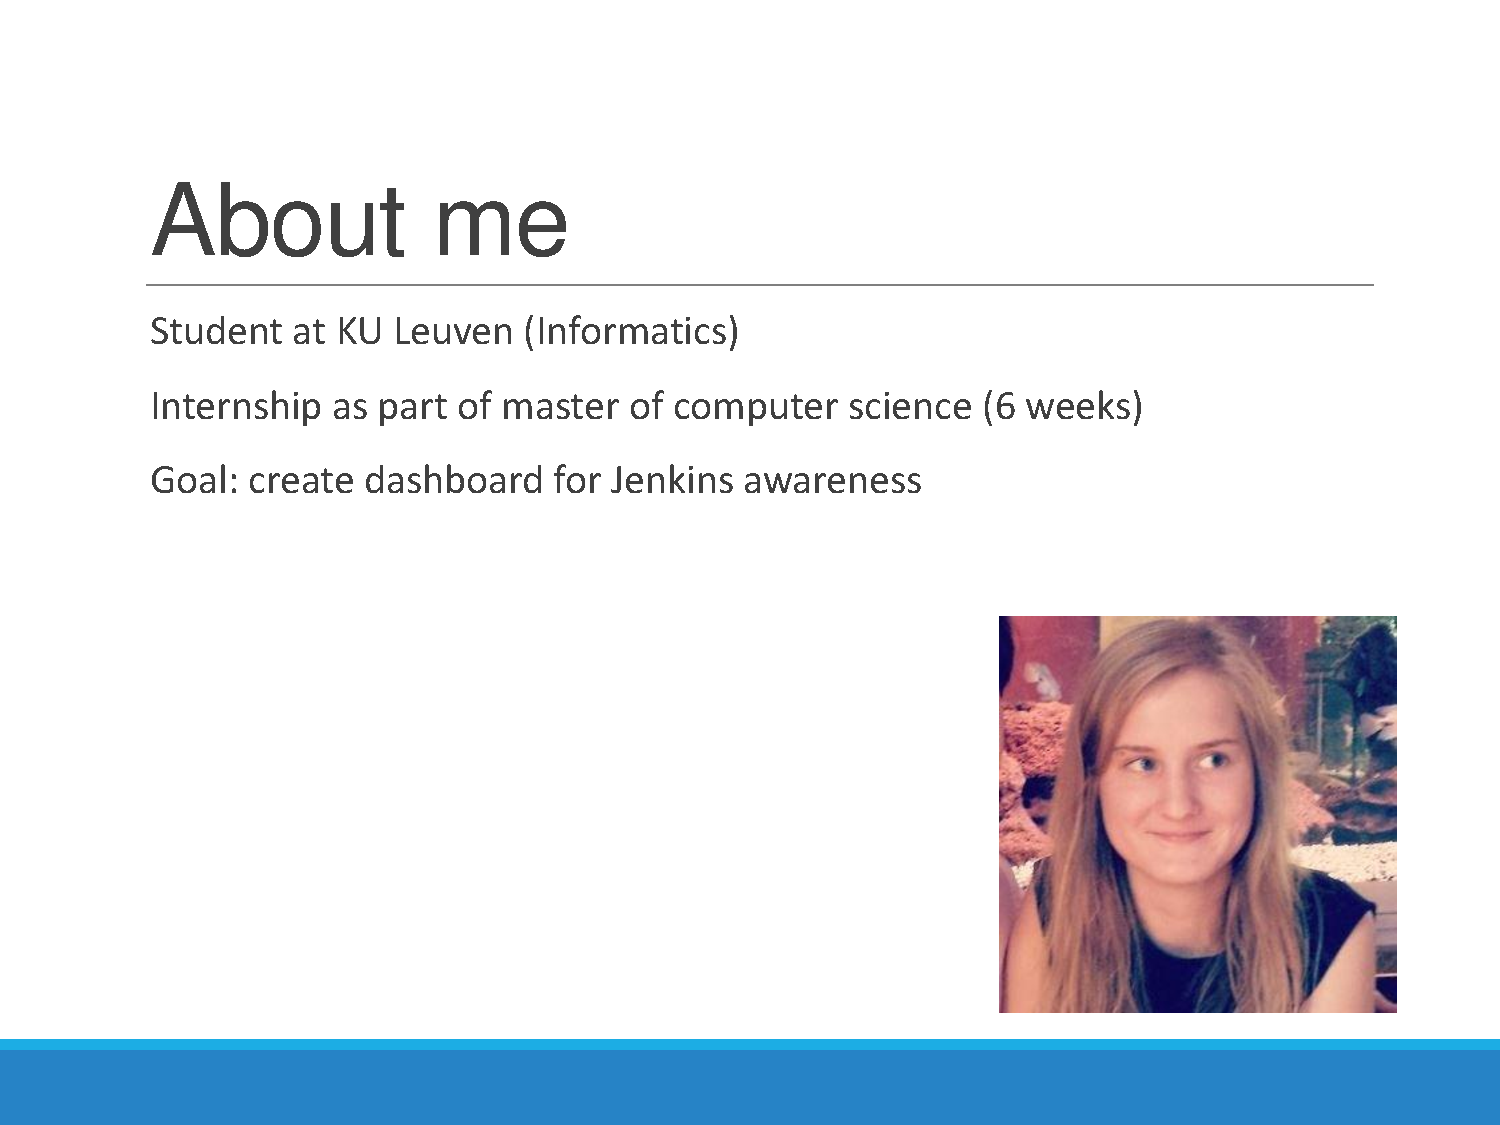
\includegraphics[width=60mm]{ppt2.pdf}
\label{jira}
\end{minipage}
\end{figure}

\begin{figure}[!h]
\centering
\begin{minipage}{0.45\textwidth}
\centering
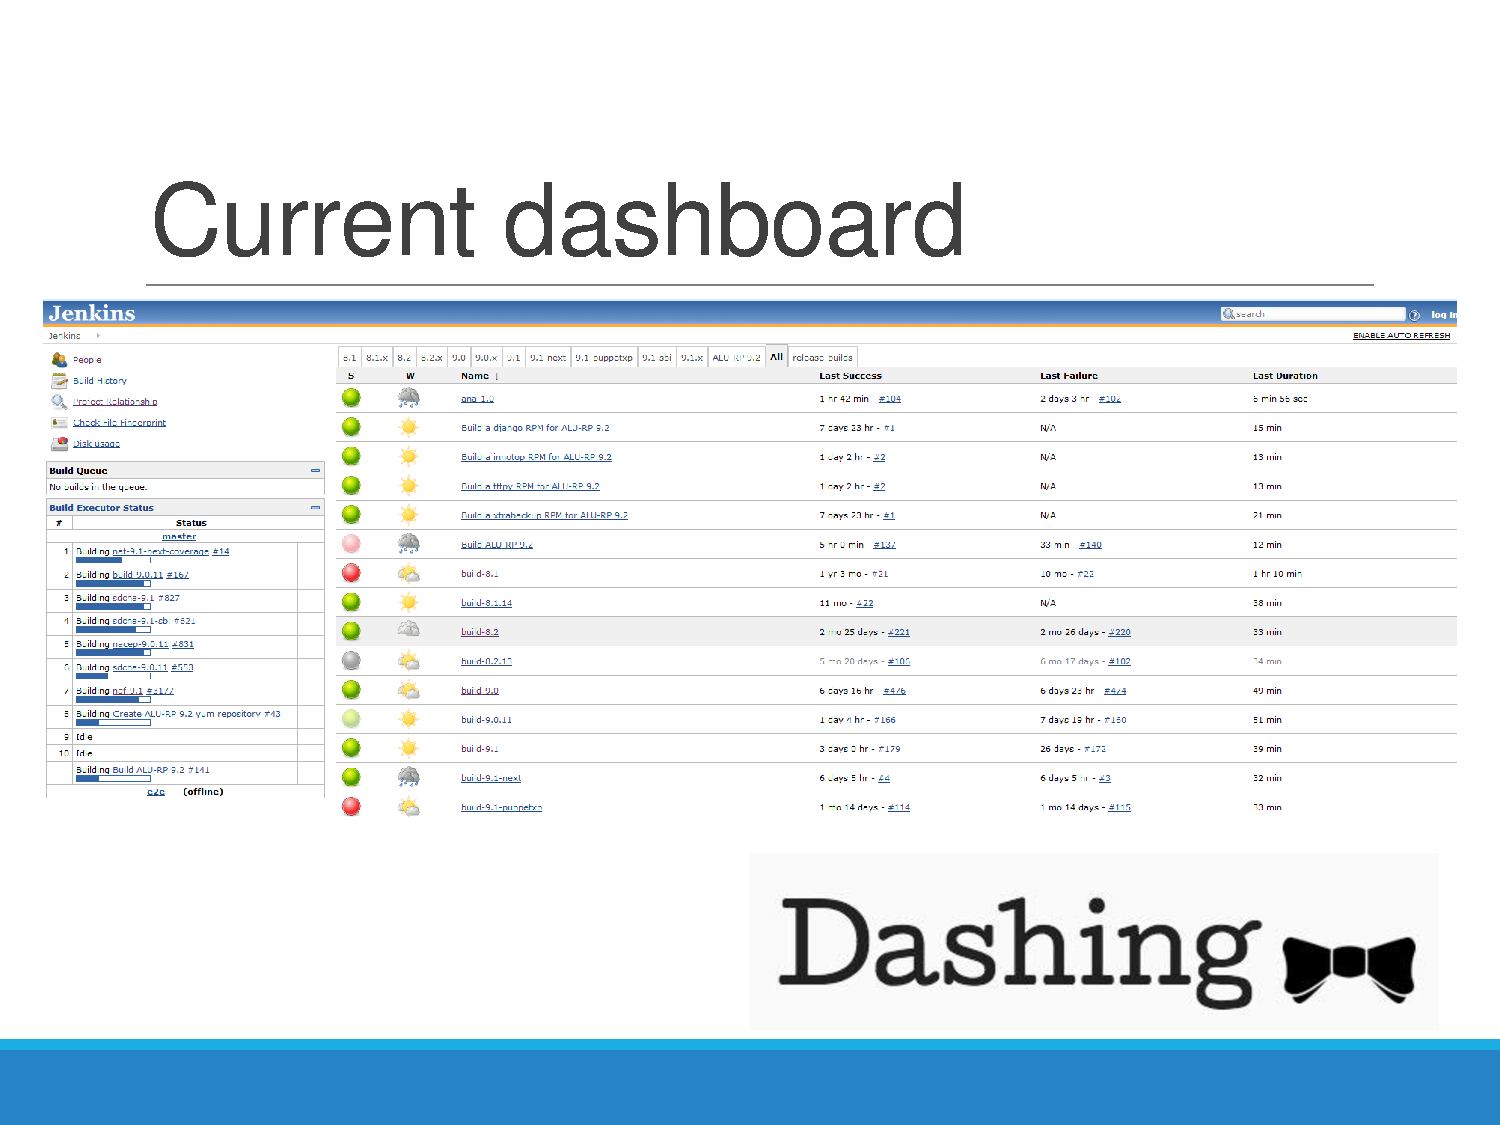
\includegraphics[width=60mm]{ppt3.pdf}
\label{standup}
\end{minipage}\hfill
\begin{minipage}{0.45\textwidth}
\centering
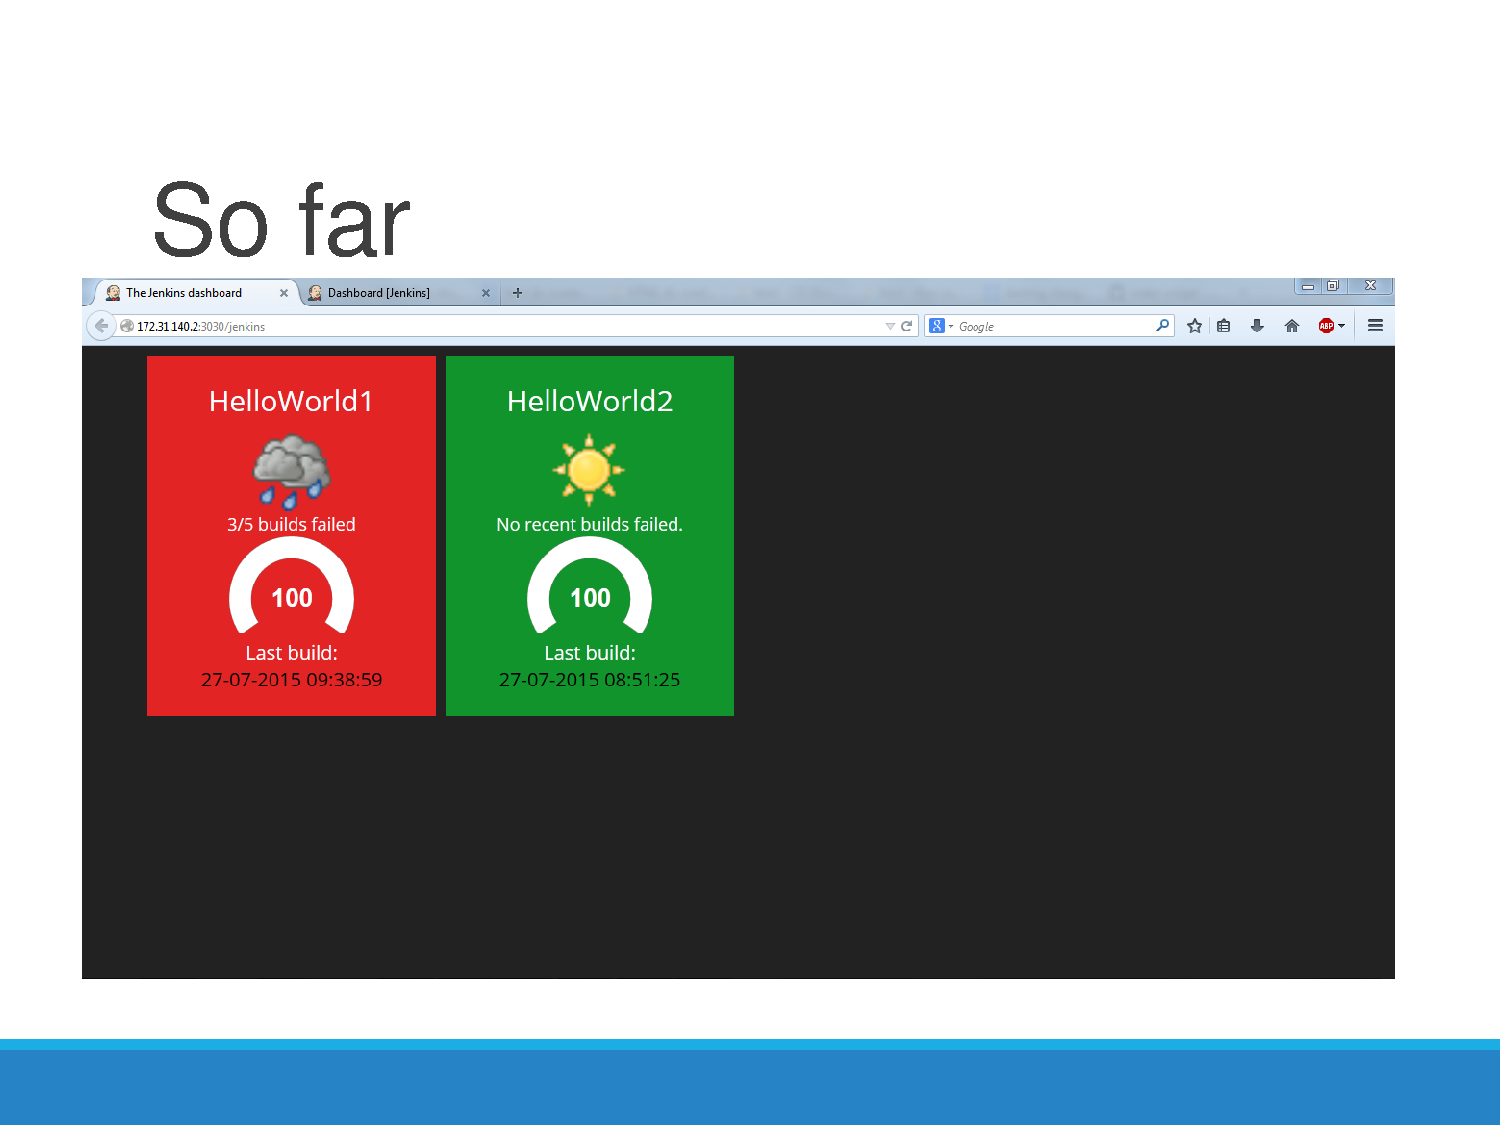
\includegraphics[width=60mm]{ppt4.pdf}
\label{jira}
\end{minipage}
\end{figure}

\clearpage

\section{Enqu\^ete 2}
\label{enquete2}
\paragraph{Enqu\^ete}
Er werd een formulier rondgegeven waarop men positieve en negatieve puntjes kon opschrijven, alsook suggesties van wat men nog graag zou zien op het dashboard.

\paragraph{Resultaten}
De positieve opmerkingen die gegeven zijn, zijn de volgende:
\begin{itemize}
\item ``The requirements are met."
\item ``Good looking/shows clearly the status of the build."
\item ``Looks good visually, nice colors, nice layout"
\item ``Very clear indication of which `project' failed. $\rightarrow$ Big title + background color."
\item ``Good look and feel. Realtime updates - very nice."
\item ``3 colors $\rightarrow$ in 1 quick view you see the complete overview."
\end{itemize}

Suggesties en negatieve puntjes die aangehaald zijn, zijn de volgende:
\begin{itemize}
\item ``Build name is in case of gray or yellow background not readable."
\item ``It does not show all the jobs. It shows maybe too much info (instead of the progress bar, you could make the background blink when a build is in progress). $\Rightarrow$ It would be better to have different `zones'. The idea would be to have jobs separated by version and some jobs `highlighted'. What matters is that when there is a release soon, we can check visually the status of all the jobs related to that release. There is no need to have all the weather info/progress for all the builds."
\item ``Build progress is less important so it can be shown less big."
\item ``Add an RSS feed for news items."
\item ``Wishlist
\begin{itemize}
\item Clicking a box should take us to the job. Top right $\rightarrow$ add link to Jenkins home, maybe the list of all jobs (the Jenkins server) - low priority.
\item Time in AM/PM.
\item The colours during `build in progress' and `build disabled' are not the same as in Jenkins.
\item Toggle button which can group per product and per release (low priority).
\item Questions:
\begin{itemize}
\item Will this survive a Jenkins upgrade?
\item How easy is it to add a new build indicator?"
\end{itemize}
\end{itemize}
\end{itemize}

Het is duidelijk dat enkele mensen nog vragen hadden bij het dashboard, dus is hen nog extra uitleg gegeven. Enkele van de voorstellen die gedaan zijn, zijn nog verder uitgewerkt.

\clearpage

\section{Bedrijfservaring: competenties}
\label{competenties}

\begin{itemize}
\item Technische competenties die ik hoop te verbeteren:
\begin{description}
\item[Bijleren over version control:] mijn taak zal erin bestaan de werking van het version control systeem overzichtelijker te maken. Op deze manier zal ik een inzicht krijgen in hoe version control gebruikt wordt in een bedrijfsomgeving.
\item[Leren werken met Jenkins:] ik had nog nooit van dit continuous integration systeem gehoord, maar het lijkt me nuttig en interessant om hierover te leren. Die ervaring kan ik eventueel gebruiken in volgende opdrachten.
\item[Mij inwerken in een reeds lopend project:] aan de KU Leuven moeten we meestal projecten vanaf nul beginnen maken, hier zal ik in een reeds bestaand project terechtkomen. Me hierin inwerken en leren hoe andere mensen de zaken aanpakken, lijkt me heel leerrijk.
\end{description}
\item Persoonlijke competenties die ik hoop te verbeteren:
\begin{description}
\item[Leren werken in grote teams:] aan de KU Leuven werk je ten hoogste met 6 mensen samen, wat al een uitdaging vormt op zich. Nu zal ik in een bedrijfsomgeving komen waarbij men met veel meer mensen samenwerkt, hieruit verwacht ik dus te leren hoe je moet samenwerken in heel grote groepen.
\item[Plannen op lange termijn:] bij projecten aan de KU Leuven kreeg je interne (kleine) deelopdrachten bij projecten, hier zal ik meer zelf moeten plannen en zien wat realiseerbaar is binnen vooropgestelde tijd.
\end{description}
\end{itemize}

\end{appendices}

\end{document}